\cleardoublepage  
\chapter{Concepts, Definitions and Notation}
\label{chap:theory}
\lhead{Chapter \ref{chap:theory}. \emph{\nameref{chap:theory}}}
This chapter gives an introduction to the base concepts used further in this report.
The chapter starts by establishing the formal definition of the problem at hand. 
Then it proceeds to detail the algorithmic and geometric concepts to be used in the different approaches described in the following chapters.
\section{Definition of Coverage}
\label{sect:problem}
Representativeness consists of finding a subset of points in a larger set. The subset chosen should be able to keep some specified properties of the original set, such as general distribution and shape. As such there can be many ways to define representativeness. For the purposes of this thesis, we will use the definition of \emph{coverage}.

Coverage measures the total volume occupied by the union of a set of shapes in space. In the 2-dimensional space, which we are using for this thesis, it means the total area occupied by a collection of 2-dimensional shapes. Since our method for representing points is the euclidean distance to other close points, the shapes in question will invariably be circles, since their circumference delimits all the possible points within a smaller distance of the given radius. As such, any point $p$ is covered by centroid $c$ if and only if it is contained in a geometric disk of the context chosen radius centred around $c$.

Although the points in this thesis represent geographic locations, the metric that would measure their distance on the surface of the globe, the geodesic distance, will not be used. The triangular inequality property does not apply to geodesic distances as a sphere (or an approximation of thereof) is not an Euclidean space, and it would add an unnecessary layer of complexity to computing the coverage.
Because of this, in this thesis, the coordinates of the points are the planar projection of the geographic coordinates to their location counterparts, as implemented by the WFS web mapping communication standard. Therefore, the Euclidean norm will be used as the spatial distance notion.

\section{Minimum Coverage Subset}

One of coverage problems approached in this thesis is the minimum coverage subset problem. Given a set of points $N$ in $\mathbb{R}^2$, we must choose a subset, $P$, that best matches our definition of representativeness.
The size of $P$, however, is constrained to a size $k$, which specifies how many points can be displayed in a section of a map.

For any point in $N$ not in $P$, there must be a point in $P$ that best represents it. This notion of representativeness may be defined by the distance, i.e.\ the point $p$ that best represents $q$ is the closest point closest to $q$, or the one that minimises euclidean distance between the pair.

Finding the most representative set $P$ in $N$ will mean that every point in $N$ will be assigned to the point in $P$ closest to it. This definition of representativeness is referred to as \emph{coverage} and the points in $P$ are called \emph{centroids}.

The coverage value of a given centroid is defined by the circle around that centroid with the radius defined by the distance between itself and the farthest non-centroid point assigned to it. The coverage value of a subset is determined by the highest coverage value of its points. It can thus be more formally described as:

\begin{equation}
\max_{n \in N}
	{\min_{p \in P}
		{\lVert p-n \rVert}
	}
\end{equation}

\noindent
where $N$ is the initial set of points in $\mathbb{R}^2$, $P$ is the centroid subset and $\lVert \cdot \rVert $ is the Euclidean distance.
The most representative subset, however, is the one with the minimum value of coverage. This means all points will be assigned to the closest centroid, minimising the coverage of all centroids and avoiding overlapping coverage areas whenever possible.
We can then finally define our problem as the minimising the coverage:

\begin{equation}
\min_{\substack{P \subseteq N\\ \lvert P \rvert = k}}{\max_{n \in N}{\min_{p \in P}{\lVert p-n \rVert}}}
\end{equation}

This is known in the field of optimisation as the \emph{k-centre} problem, and is an example of a facility location problem \cite{thisfref}. Figure \ref{fig:cov} shows two possible centroid assignments, each with its own value of coverage, $d$.

\begin{figure}[H]
	\centering
	\begin{minipage}{0.45\linewidth}
		\centering
		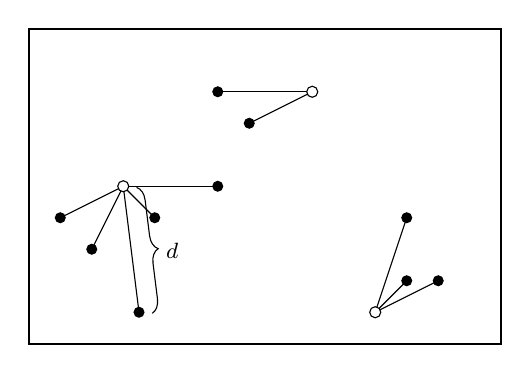
\begin{tikzpicture}[scale=0.4]
		
		\draw [<->,thick] (0,0) rectangle (15,10) {};
		%centroids
		
		%Left Group
%		\fill ( 7,7) circle (5pt);
		\fill ( 1,4) circle (5pt);
		\fill ( 4,4) circle (5pt);
		\fill ( 2,3) circle (5pt);
		\fill (3.5,1) circle (5pt);
		\fill ( 6,5) circle (5pt);
		
		%Middle Group
		
		\fill ( 7,7) circle (5pt);
		\fill ( 6,8) circle (5pt);
		
		%Right Group
		\fill (12,2) circle (5pt);
		\fill (12,4) circle (5pt);
		\fill (13,2) circle (5pt);
		
		%Lines
		\draw [-] (1,4) -- (3,5);
		\draw [-] (4,4) -- (3,5);
		\draw [-] (2,3) -- (3,5);
		\draw [-] (3.5,1) -- (3,5);
		\draw [-] (6,5) -- (3,5);
		
		\draw [-] (7,7) -- (9,8);
		\draw [-] (6,8) -- (9,8);
		
		\draw [-] (12,2) -- (11,1);
		\draw [-] (12,4) -- (11,1);
		\draw [-] (13,2) -- (11,1);
		\fill [white] (11,1) circle (5pt);
		\fill [white] ( 3,5) circle (5pt);
		\fill [white] ( 9,8) circle (5pt);
		
		\draw (11,1) circle (5pt);
		\draw ( 3,5) circle (5pt);
		\draw ( 9,8) circle (5pt);
		
		\draw [decorate,decoration={brace,amplitude=5pt},xshift=12pt,yshift=-1pt]
		(3,5) -- (3.5,1)node [black,midway,xshift=10pt] {\footnotesize$d$};
		\end{tikzpicture}
		\caption*{Non-Optimal Assignment}
		\label{fig:badcov}
	\end{minipage}
	\begin{minipage}{0.45\linewidth}
		\centering
		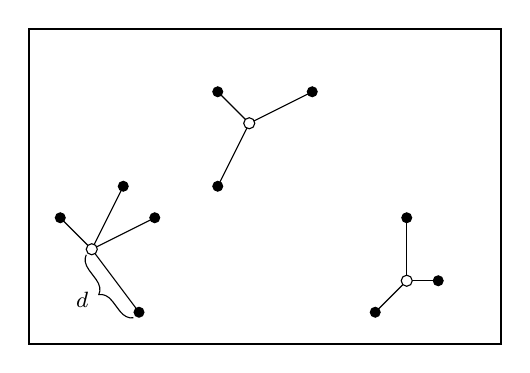
\begin{tikzpicture}[scale=0.4]
		
		\draw [<->,thick] (0,0) rectangle (15,10) {};
		%centroids
		
		%Left Group
		\fill ( 1,4) circle (5pt);
		\fill ( 4,4) circle (5pt);
		\fill ( 3,5) circle (5pt);
		\fill (3.5,1) circle (5pt);
		
		%Middle Group
		\fill ( 6,5) circle (5pt);
		\fill ( 9,8) circle (5pt);
		\fill ( 6,8) circle (5pt);
		
		%Right Group
		\fill (11,1) circle (5pt);
		\fill (12,4) circle (5pt);
		\fill (13,2) circle (5pt);
		
		%\pause
		%Lines
		\draw [-] (1,4) -- (2,3);
		\draw [-] (4,4) -- (2,3);
		\draw [-] (3,5) -- (2,3);
		\draw [-] (3.5,1) -- (2,3);
		
		\draw [-] (6,5) -- (7,7);
		\draw [-] (9,8) -- (7,7);
		\draw [-] (6,8) -- (7,7);
		
		\draw [-] (11,1) -- (12,2);
		\draw [-] (12,4) -- (12,2);
		\draw [-] (13,2) -- (12,2);
		
		\fill [white] ( 2,3) circle (5pt);
		\fill [white] (12,2) circle (5pt);
		\fill [white] ( 7,7) circle (5pt);
		
		\draw ( 2,3) circle (5pt);
		\draw (12,2) circle (5pt);
		\draw ( 7,7) circle (5pt);
		
		%Circles
		%\draw [dashed] (2,3) circle (2.5);
		%\draw [dashed] (7,7) circle (2.236);
		%\draw [dashed] (12,2) circle (2);
		%\pause
		\draw [decorate,decoration={brace,amplitude=5pt},xshift=-5pt,yshift=-5pt]
		(3.5,1) -- (2,3)node [black,midway,xshift=-10pt,yshift=-5pt] {\footnotesize$d$};
		\end{tikzpicture}		
		\caption*{Optimal Assignment}
		\label{fig:goodcov}
	\end{minipage}
	\caption{Different assignments for the same set of points}
	\label{fig:cov}
\end{figure}

For the 1-dimensional case, the minimum coverage value can be calculated in polynomial time \cite{dvaz}. However, for any other number of dimensions it is a \emph{NP-hard} problem, and cannot be solved in polynomial time \cite{complex}.

%\section{k-Centre}
The \emph{k-centre} problem is a well known problem in the optimisation field of study. As such, several approaches have been explored over the years. In the following, two important approaches are described: an Integer Linear Programming approach and an Incremental Approach.

\subsection{Integer Linear Programming Formulation}
\label{alg:ilp}

A simple and straight-forward approach to the problem is to model it in  integer linear programming as follows:
\begin{align}
\text{minimise}   \quad& D				   &\\
\text{subject to} \quad
& \sum\limits_{j=1}^{N}{y_j} = k 
& 							\label{ilp:1}\\
& \sum\limits_{j=1}^{N}{x_{ij}}	= 1   
& i=1,\ldots,N 				\label{ilp:2}\\
& \sum\limits_{j=1}^{N}{d_{ij} x_{ij}} \leq D
& i=1,\ldots,N				\label{ilp:3}\\
& x_{ij} \leq y_{j}				   
& i=1,\ldots,N;j=1,\ldots,N	\label{ilp:4}\\
& x_{ij},y_{j} \in \{0,1\}
& i=1,\ldots,N;j=1,\ldots,N \label{ilp:5}
\end{align}
In this formulation, $y_j = 1$ if point $j$ is a centroid and $y_j = 0$ if it is a non-centroid;
$x_{ij} = 1$ if the point $i$ is assigned to the centroid $j$, and $x_{ij}=0$ otherwise;
$d_{ij}$ is the Euclidean distance between points $i$ and $j$.
Constraint \eqref{ilp:1} ensures that $k$ centroids are chosen.
Constraint \eqref{ilp:2} limits the assignment of one point to more than one centroid.
Constraint \eqref{ilp:3} ensures that all active distances are lower than the limit we are minimising.
Constraint \eqref{ilp:4} limits points to being assigned only to centroids, where $y_j=1$.
Constraint \eqref{ilp:5} defines both $x_{ij}$ and $y_j$ as binary variables, in order to properly represent selection and assignment.

It is worth noting that this formulation minimises the objective function by selecting the best possible set of centroids, but it only minimises the maximum coverage. This way, only the farthest point from its centroid has the guarantee that it is connected to its closest centroid.
Every other point, however, can be linked to any centroid so long as it is closer to it than the distance defined by the objective function, since $d_{ij}x_{ij}$ only has to be lower than $D$, but not include the lowest possible values.
Likewise, it can also produce the result where one centroid is assigned to another centroid as opposed to itself, as long as they are close enough together and it does not affect the coverage of the whole set.
These cases have no effect on the outcome of the final coverage value or the centroid selection, but are rather counter-productive, since we want to minimize the coverage of all centroids, with minimal overlapping of the covered areas.

In order to best display the results, a simple post-processing step can be applied, where each point will be strictly assigned to the closest centroid. This can be easily computed in $\mathcal{O}((N-k)k)$ time in case there is a need for a clearer display of the assignment.

Other more elaborate formulations can be used. \citet{linearprog} explore a new formulation to obtain tighter bounds in the LP relaxation. They also limit the values that the solution can take by enumerating all different values of distances between points and sorting them in decreasing order.

\subsection{Local Search Approach \incomp{\#\# Mudar para o capitulo do B\&B??}}
\citet{incrementalcov} solve the \emph{k-centre} problem heuristically using local search. Their method describes algorithms to incrementally insert and remove centroids from a set of points, and update the centroid assignment only in the geometrical area surrounding the changed centroid. This method allows for small modifications on an already valid solution, until a similar solution is deemed optimal is found. It can be used as a fast way to calculate neighbour solutions to be used in heuristic approaches to the \emph{k-centre} problem.

In order to minimise computation time, \citet{incrementalcov} maintain the selected centroids in a \emph{k-d tree}. Using a \emph{k-d tree} reduces the number of comparisons needed for the step of point location in the algorithm. To keep the \emph{k-d trees} from loosing efficiency in insertions and removal of points, the trees need to be balanced from time to time. Calculating the optimal time interval to balance the \emph{k-d tree} has to be done \emph{a priori} and can affect the performance of the algorithm.

The structures and incremental procedures can be used with enumeration algorithms in order to obtain the global optimum solution.

\section{Geometric Disk Coverage}
\label{ilp2}
Another coverage problem considered in this thesis is the geometric disk coverage problem. Given a set of objects $O$ and a fixed distance $d$, find the set of disks of radius $d$ centred around a set of centroids $P$, such that all points in $O$ are covered. The cardinality of $P$ must be as small as possible. In the most general variation of this problem, and in the problem at hand, $O$ is the original set of 2-dimensional points $N$ as described above. Added to this, there is the restriction that $C$ must be contained in $N$. This is also a variation of a facility location problem, and shares some similarities with the minimum coverage subset. 

\subsection{Integer Linear Programming}
The geometric distance cover problem can be seen as a dual problem to the minimum cover subset. In fact, an Integer Linear Programming formulation can be obtained by swapping the objective function for one of the constraints:

\begin{align}
\text{minimise}   \quad& k							   &\\
\text{subject to} \quad
& \sum\limits_{j=1}^{N}{y_j} \leq k 
& 							\label{ilp2:1}\\
& \sum\limits_{j=1}^{N}{x_{ij}}	= 1   
& i=1,\ldots,N 				\label{ilp2:2}\\
& \sum\limits_{j=1}^{N}{d_{ij} x_{ij}} \leq D
& i=1,\ldots,N				\label{ilp2:3}\\
& x_{ij} \leq y_{j}				   
& i=1,\ldots,N;j=1,\ldots,N	\label{ilp2:4}\\
& x_{ij},y_{j} \in \{0,1\}
& i=1,\ldots,N;j=1,\ldots,N \label{ilp2:5}
\end{align}
In this formulation, the value for the minimum distance $D$ is given as a parameter and $k$ is the value minimized. The value for $y_j = 1$ if point $j$ is a centroid and $y_j = 0$ if it is a non-centroid;
$x_{ij} = 1$ if the point $i$ is assigned to the centroid $j$, and $x_{ij}=0$ otherwise;
$d_{ij}$ is the Euclidean distance between points $i$ and $j$.
Constraint \eqref{ilp2:1} ensures that $k$ or less centroids are chosen.
Constraint \eqref{ilp2:2} limits the assignment of one point to more than one centroid.
Constraint \eqref{ilp2:3} ensures that all active distances are lower than the limit we are minimising.
Constraint \eqref{ilp2:4} limits points to being assigned only to centroids, where $y_j=1$.
Constraint \eqref{ilp2:5} defines both $x_{ij}$ and $y_j$ as binary variables, in order to properly represent selection and assignment.

\section{Algorithmic Concepts}
\subsection{Branch-and-Bound}
Minimising coverage, as shown, is a \emph{NP-hard} combinatorial problem \cite{complex}. One possible way of solving the problem is to use implicit enumeration algorithms such as \emph{Branch-and-Bound} algorithms.
These algorithms solve the problems by recursively dividing the solution set in half, thus \emph{branching} it into a rooted binary tree.
At each step of the subdivision, it then calculates the upper and lower bounds for the best possible value for the space of solutions considered at that node. This step is called \emph{bounding}.
In the case of a minimisation problem, it would be the upper and lower bounds for minimum possible value for the objective function in the current node. These values are then compared with the best ones already calculated in other branches of the recursive tree, and updated if better.

The bounds can be used to \emph{prune} the search tree. This can be done when the branch-and-bound algorithm arrives at a node where the lower bound is larger than the best calculated upper bound. At this point, no further search within the branch is required, as there is no solution in the current branch better than one that has already been calculated. 
In the case that the global upper and lower bound meet, the algorithm has arrived at the best possible solution, and no further computation must be done.

These algorithms are very common in the field of optimisation and can be very efficient, but their performance depends on the complexity and tightness of its bounds. Tighter bounds accelerate the process, but are usually slower to compute, so a compromise has to be made in order to obtain the fastest possible algorithm.

\subsection{Approximation Algorithms}
Optimal solution algorithms, even very optimized ones, are oftentimes still too inefficient to be used in any practical, time constrained application. One possible strategy to solve an \emph{NP-hard} problem is to use an \emph{approximation algorithm}.

Approximation algorithms do not compute the optimal solution to a given problem. Instead, for the sake of time efficiency, these algorithms are designed to compute a solution that differs from the optimal by a given predictable factor. For example, a 2-approximation algorithm for a minimising problem will not compute any solution that is more than double the optimal value for any given input. By compromising the quality of the solution, the algorithms can be run in polynomial time.

\subsubsection*{Set Cover}
One example of an approximation algorithm is the greedy approach to solving the \emph{Set Cover} problem. Given a Universe $U$ of $n$ elements, and sets $S_1,\dotsc,S_k \subseteq U$, one must find the smallest cardinality collection of sets whose union covers $U$.

Calculating the optimal solution to the Set Cover problem is \emph{NP-hard}, and thus cannot be solved in polynomial time. However, by using the greedy approach of iteratively picking the set that contains the most uncovered points, it is possible to achieve an approximated solution in polynomial time. Assuming the instance of the problem has an optimal solution of $m$ sets, the greedy algorithm guarantees that its solution is bound above by $m \log_e n$.

\begin{theorem}
The greedy algorithm for the Set Cover can find a collection with at most $m \log_e n$ sets, where $m$ is the optimal number, and $n$ is the number of elements covered by all sets.

\begin{proof}
Let the universe $U$ contain $n$ points, which can be covered by at least $m$ sets. The first set picked by the algorithm has size at least $n/m$. The number of elements of $U$ left to cover $n_1$ is

\begin{equation}
n_1 \leq n - n/m = n(1-1/m)
\end{equation}

The remaining sets must contain at least $n_1/(m-1)$ elements, otherwise the optimal solution would have to contain more than $m$ sets. By iteratively calling the same process, the number of sets at stage $i$ is given by

\begin{align}
\begin{aligned}
n_{i+1} & \leq n_i(1-1/m) \\ 
n_{i+1} & \leq n(1-1/m)^{i+1}
\end{aligned}
\end{align}
If it takes $k$ stages for the greedy algorithm to cover $U$, then $n_k \leq n(1-1/m)^1$ needs to be less than 1.
\begin{align}
\begin{aligned}
n(1-1/m)^k & < 1 \\
n(1-1/m)^{m \frac{k}{m}} & < 1\\
(1-1/m)^{m \frac{k}{m}} & < 1/n\\
e^{-\frac{k}{m}} & < 1/n \ldots (1-x)^\frac{1}{x} \approx 1/e\\
k/m & > \log_e n \\
k & < m\log_e n
\end{aligned}
\end{align}
This means that the size of the collection of sets picked by the greedy algorithm is bound above by $m \log_e n$, which gives the greedy algorithm a $\bigo(\log_e n)$ approximation to the optimal solution.

\end{proof}
\end{theorem}



\section{Geometric Concepts and Geometric Structures}
In the following, we explain some geometric concepts that are used in the following chapters, in order to simplify the explanation of more complex algorithms in further chapters.
\subsection{Nearest Neighbour Search and Point Location}
A common concept in computational geometry is point location. A point location algorithm finds the region on a plane that contains a given point $p$. Depending on the nature and shape of the regions, point location algorithms may differ in approach. In this thesis, most point location problems consist of finding the closest centroid to a given point, i.e.\ a nearest neighbour search algorithm.

Given a point $p$, a \emph{nearest neighbour search} algorithm returns the closest point to $p$ in a given set. Since we need to find the closest centroid to a given point in order to find the correct coverage value, this operation will be one of the most used, and  so we need a fast and flexible way of determining which of the centroids is closest, in order to reduce computational overhead. 

Point location algorithms direct the nearest neighbour search to smaller regions, bypassing any regions that are too distant from $p$, thus reducing the number of calculations necessary to get the proper point location.
Common structures used for point location are \emph{k-d trees} as described in \citet{incrementalcov}. A \emph{k-d tree} partitions the space using a divide and conquer approach to define orthogonally aligned half-planes. This approach takes $\bigo(\log{n})$ time to achieve point location queries. However, a \emph{k-d tree} needs to be periodically updated in order to keep its efficiency and cannot be constructed or deconstructed incrementally without considering this overhead.

\subsection{\textit{k}-Dimensional Trees}

A \textit{k}-dimensional tree, or \kdtree, is a space partitioning structure used for point location and nearest neighbour queries. A \kdtree is a binary tree, which each of whose nodes represents an axis-aligned hyper-rectangle. Each node specifies an axis and splits the set of points based on whether their coordinate along that axis is greater than or less than a particular value. The axis chosen to split each subgroup is chosen via a rotation system, which in the 2-dimensional space means that each level alternates between the vertical and horizontal axis.

During construction, the splitting point is chosen to be the point whose relevant coordinate best divides the group intro two subgroups. The best possible choice for the splitting point at each level is the point which has the median of the relevant coordinate in the group. This ensures that each node divides the number of points in half for so that the resulting tree becomes balanced, and that each point is reachable by performing $\bigo(\log{n})$ operations.

\begin{figure}[H]
	\begin{center}
		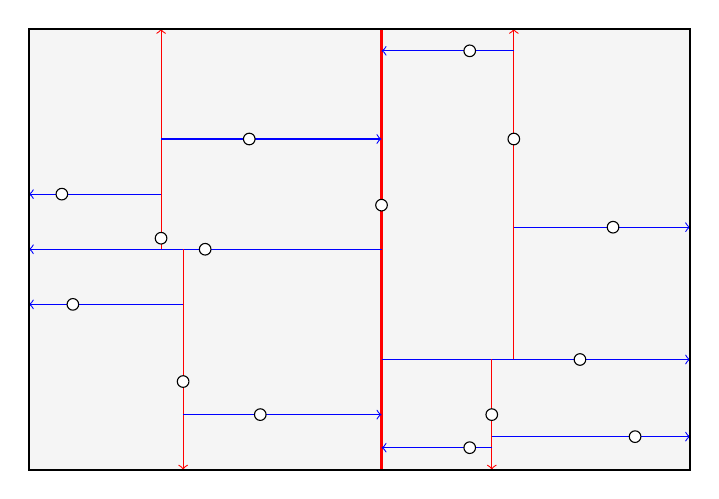
\begin{tikzpicture}[scale=1.4]
			\fill[lightgray!15] (0,0) rectangle (6,4);
			\draw [red,thick](3.2,0) -- (3.2,4);
			\fill[white,draw=black] (3.2,2.4) circle (1.5pt);
				\draw [blue,->](3.2,1) -- (6,1);
				\fill[white,draw=black] (5,1) circle (1.5pt);
					\draw [red,<-](4.2,0) -- (4.2,1);
					\fill[white,draw=black] (4.2,0.5) circle (1.5pt);
						\draw [blue,<-](3.2,0.2) -- (4.2,0.2);
						\fill[white,draw=black] (4,0.2) circle (1.5pt);
						\draw [blue,->](4.2,0.3) -- (6,0.3);
						\fill[white,draw=black] (5.5,0.3) circle (1.5pt);
					\draw [red,->](4.4,1) -- (4.4,4);
					\fill[white,draw=black] (4.4,3) circle (1.5pt);
						\draw [blue,<-](3.2,3.8) -- (4.4,3.8);
						\fill[white,draw=black] (4,3.8) circle (1.5pt);
						\draw [blue,->](4.4,2.2) -- (6,2.2);
						\fill[white,draw=black] (5.3,2.2) circle (1.5pt);
				\draw [blue,<-](0,2) -- (3.2,2);
				\fill[white,draw=black] (1.6,2) circle (1.5pt);
					\draw [red,->](1.2,2) -- (1.2,4);
					\fill[white,draw=black] (1.2,2.1) circle (1.5pt);
						\draw [blue,->](1.2,3) -- (3.2,3);
						\fill[white,draw=black] (2,3) circle (1.5pt);
						\draw [blue,<-](0,2.5) -- (1.2,2.5);
						\fill[white,draw=black] (0.3,2.5) circle (1.5pt);
					\draw [red,<-](1.4,0) -- (1.4,2);
					\fill[white,draw=black] (1.4,0.8) circle (1.5pt);
						\draw [blue,->](1.4,0.5) -- (3.2,0.5);
						\fill[white,draw=black] (2.1,0.5) circle (1.5pt);
						\draw [blue,<-](0,1.5) -- (1.4,1.5);
						\fill[white,draw=black] (0.4,1.5) circle (1.5pt);
						
			\draw[thick] (0,0) rectangle (6,4);
		\end{tikzpicture}
	\end{center}
	\caption{Example of a \kdTree}
	\label{fig:kd1}
\end{figure}
\subsubsection*{Construction}
Constructing a \kdtree requires selecting a pivot, which divides the set into two groups: the points whose relevant coordinate is smaller than the pivot, the points whose relevant coordinate is larger than the pivot. The same process is then repeated recursively for each of the groups, alternating the relevant coordinate between both axes. Each recursive call fixes one pivot, which ideally will contain the median value of the relevant coordinate. The time complexity of the construction of a \kdtree relies on the pivot selection function. Calculating the median usually requires sorting a list of $n$ and then picking the $n/2$th element. Since sorting algorithms typically take $\bigo(n \log{n})$, building a \kdtree would take $\bigo(n^2)$ time. To achieve better time complexity and performance the median of medians algorithm described in \ref{median} can be used.

Even though the median of medians algorithm does not necessarily return the actual median, the query complexity in a \kdtree constructed using this still achieves the $\bigo(\log{n})$. This occurs because the median of medians always outputs a value between the $30$th and $70$th percentile. This guarantees that at each level of the \kdtree the group of points covered by each of the children nodes is substantially smaller than the parent node by a constant factor, and there will never be a redundant node that covers the same set of points the parent does. At each level of a given query, each decision discards at least 30\% of the points, maintaining the $\bigo(\log{n})$ time complexity \cite{kdmedian}.

\subsection{Orthogonal Aligned Range Search}
Some geometric algorithms require knowing which subset of points are contained in a given area. This operation is known as range search. A range search can be used to find all the neighbours of a given point that are within a fixed radius. This is most efficiently done by performing a orthogonally aligned range search on the square that encloses the range circle. Performing a orthogonally aligned range search query on a set of points can be done using a \kdtree structure or a line sweep.

\subsubsection*{\kdTree Range Search}
\label{sect:kdrs}
Performing a range search on a \kdtree can be done recursively. Each level of the \kdtree alternates the dimension it divides the plane in. Starting at the root, only the sides (left and/or right) that intersect the queried rectangle are checked for points contained inside it. Figure \ref{fig:kdrs} illustrates a 2-dimensional \kdtree.

\begin{figure}[!h]
	\begin{center}
		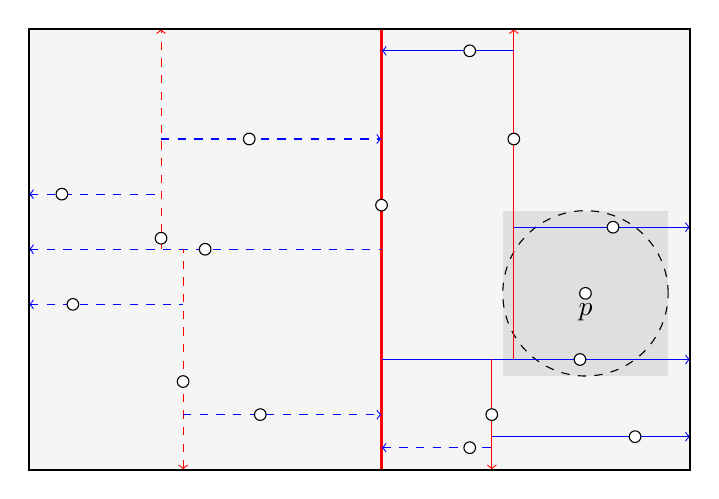
\begin{tikzpicture}[scale=1.4]
		\fill[lightgray!15] (0,0) rectangle (6,4);
		\fill[lightgray!50] (4.3,0.85) rectangle (5.8,2.35);
		\draw[dashed](5.05,1.6) circle(0.75);
		\fill[white,draw=black] (5.05,1.6) circle(1.5pt);
		\node[below] at (5.05,1.6) {$\tiny p$};
		
		\draw [red,thick](3.2,0) -- (3.2,4);
		\fill[white,draw=black] (3.2,2.4) circle (1.5pt);
		\draw [blue,->](3.2,1) -- (6,1);
		\fill[white,draw=black] (5,1) circle (1.5pt);
		\draw [red,<-](4.2,0) -- (4.2,1);
		\fill[white,draw=black] (4.2,0.5) circle (1.5pt);
		\draw [blue,<-,dashed](3.2,0.2) -- (4.2,0.2);
		\fill[white,draw=black] (4,0.2) circle (1.5pt);
		\draw [blue,->](4.2,0.3) -- (6,0.3);
		\fill[white,draw=black] (5.5,0.3) circle (1.5pt);
		\draw [red,->](4.4,1) -- (4.4,4);
		\fill[white,draw=black] (4.4,3) circle (1.5pt);
		\draw [blue,<-](3.2,3.8) -- (4.4,3.8);
		\fill[white,draw=black] (4,3.8) circle (1.5pt);
		\draw [blue,->](4.4,2.2) -- (6,2.2);
		\fill[white,draw=black] (5.3,2.2) circle (1.5pt);
		\draw [blue,<-,dashed](0,2) -- (3.2,2);
		\fill[white,draw=black] (1.6,2) circle (1.5pt);
		\draw [red,->,dashed](1.2,2) -- (1.2,4);
		\fill[white,draw=black] (1.2,2.1) circle (1.5pt);
		\draw [blue,->,dashed](1.2,3) -- (3.2,3);
		\fill[white,draw=black] (2,3) circle (1.5pt);
		\draw [blue,<-,dashed](0,2.5) -- (1.2,2.5);
		\fill[white,draw=black] (0.3,2.5) circle (1.5pt);
		\draw [red,<-,dashed](1.4,0) -- (1.4,2);
		\fill[white,draw=black] (1.4,0.8) circle (1.5pt);
		\draw [blue,->,dashed](1.4,0.5) -- (3.2,0.5);
		\fill[white,draw=black] (2.1,0.5) circle (1.5pt);
		\draw [blue,<-,dashed](0,1.5) -- (1.4,1.5);
		\fill[white,draw=black] (0.4,1.5) circle (1.5pt);
		\draw[thick] (0,0) rectangle (6,4);
		\end{tikzpicture}
	\end{center}
	\caption[Example of a range search query on a \kdTree] {The dashed lines are never queried, since the rectangle does not intercept their parent. This query searches for all points within a fixed distance of $p$.}
	\label{fig:kdrs}
\end{figure}

If the rectangle queried is small enough, this method eliminates most candidates from being checked, thus improving on a brute force algorithm. However, since the rectancle can be big enough to cover all points, the worst case is still the same, since returning the whole set of points will never take less than linear time to compute. The expected time complexity is given by $\bigo(2N^{\frac{1}{2}})$ for queries in two dimension \cite{kdrange}.
	
If the rectangle to be queried is a square of side $2d$ centred around a given point $p$, this query can be used to limit the number of points to be tested for being within a fixed radius $d$ around $p$.


\subsubsection*{Line Sweep Range Search}
\label{sect:lsrs}
A Line Sweep method can also be used to find all the points in a orthogonally aligned rectangle. The line sweep algorithm starts by sorting the points on one of the coordinates, usually the $x$ coordinate. Then, an imaginary vertical line starts sweeping each pair of points, until the distance between them is larger than the width of the rectangle, when the operation can be stopped.
	
\begin{figure}[!h]
\begin{center}
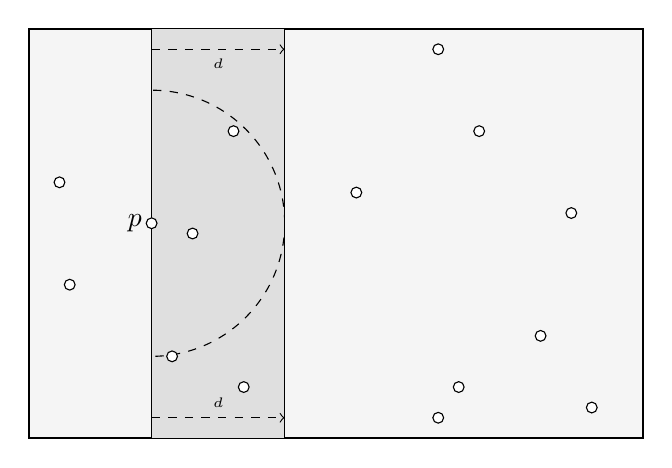
\begin{tikzpicture}[scale=1.3]
	\fill[lightgray!15,draw=black,thick] (0,0) rectangle (6,4);
	\fill[lightgray!50,draw=black] (1.2,0) rectangle (2.5,4);
	\begin{scope}
	\clip (1.2,0) rectangle (2.5,4);
	\draw[dashed](1.2,2.1) circle (1.3);
	\end{scope}
	
	\draw [dashed,->](1.2,0.2) -- node[above]{\tiny$d$}(2.5,0.2);

	\draw [dashed,->](1.2,3.8) -- node[below]{\tiny$d$}(2.5,3.8);

	\node[left] at (1.2,2.1) {$\tiny p$};

	\fill[white,draw=black] (3.2,2.4) circle (1.5pt);
	\fill[white,draw=black] (5,1) circle (1.5pt);		
	\fill[white,draw=black] (4.2,0.5) circle (1.5pt);
	\fill[white,draw=black] (4,0.2) circle (1.5pt);
	\fill[white,draw=black] (5.5,0.3) circle (1.5pt);
	\fill[white,draw=black] (4.4,3) circle (1.5pt);
	\fill[white,draw=black] (4,3.8) circle (1.5pt);
	\fill[white,draw=black] (5.3,2.2) circle (1.5pt);
	\fill[white,draw=black] (1.6,2) circle (1.5pt);
	\fill[white,draw=black] (1.2,2.1) circle (1.5pt);
	\fill[white,draw=black] (2,3) circle (1.5pt);
	\fill[white,draw=black] (0.3,2.5) circle (1.5pt);
	\fill[white,draw=black] (1.4,0.8) circle (1.5pt);
	\fill[white,draw=black] (2.1,0.5) circle (1.5pt);
	\fill[white,draw=black] (0.4,1.5) circle (1.5pt);

\end{tikzpicture}
\end{center}
\label{fig:ls1}
\end{figure}

If the rectangle to be queried is a square of side $2d$ centred around a given point $p$, this query can be used to limit the number of points to be tested for being within a fixed radius $d$ around $p$. Doing so is a matter of performing the line sweep twice, once in each direction. A special property of this algorithm is that it can find all neighbours of all points within a distance by performing the sweep starting on every point. This method does not require both directions to be swept, since this definition of neighbourhood is mutual. So if $q$ is a neighbour to $q$, then $q$ is a neighbour to $p$. Each of the queries still take $\bigo(n)$  time for each point, since each swipe can contain all of the other points

\subsection{Voronoi Diagrams}
Voronoi diagrams \cite{tricard2} partition the space into regions, which are defined by the set of points in the space that are closest to a subset of those points. Definitions of distance and space may vary, but on our case we will consider the $\mathbb{R}^2$ plane and the Euclidean distance.
Figure \ref{fig:vd1} shows a partitioning of a plane using a Voronoi Diagram for a set of points:
\begin{figure}[H]
	\begin{center}
		\begin{tikzpicture}[scale=0.4]
		%\draw [<->,thick] (0,10) node (yaxis) [left] {}
		%|- (15,0) node (xaxis) [below] {};
		%centroids
		\fill ( 2, 7) circle (3pt);
		\fill ( 5, 3) circle (3pt);
		\fill ( 6, 9) circle (3pt);
		\fill ( 8, 4) circle (3pt);
		\fill (10, 1) circle (3pt);
		\fill (11, 8) circle (3pt);
		\fill (13, 5) circle (3pt);
		\fill (13,10) circle (3pt);
		\fill (15, 7) circle (3pt);
		\fill (16, 3) circle (3pt);
		
		\draw [-] ( 5.6764, 5.9706) -- ( 4.9545, 6.0909);
		\draw [-] ( 5.6764, 5.9706) -- ( 8.1956, 6.9783);
		\draw [-] (10.3235, 5.3824) -- ( 8.1956, 6.9783);
		\draw [-] (10.3235, 5.3824) -- (10.6765, 3.6176);
		\draw [-] ( 7.2272, 1.3182) -- (10.6765, 3.6176);
		\draw [-] ( 7.2272, 1.3182) -- ( 5.6764, 5.9706);
		\draw [-] (13.0556, 1.3182) -- (10.6765, 3.6176);
		\draw [-] (13.0556, 1.3182) -- (15.1000, 4.9000);
		\draw [-] (12.9000, 7.1000) -- (15.1000, 4.9000);
		\draw [-] (12.9000, 7.1000) -- (10.3235, 5.3824);
		\draw [-] (12.9000, 7.1000) -- (13.1000, 7.9000);
		\draw [-] ( 9.1667,11.8333) -- (13.1000, 7.9000);
		\draw [-] ( 9.1667,11.8333) -- ( 8.1956, 6.9783);

		\draw [-,dashed] ( 4.9545, 6.0909) -- (2 , 12);
		\draw [-,dashed] ( 4.9545, 6.0909) -- (0, 2.375);
		\draw [-,dashed] ( 7.2272, 1.3182) -- ( 6.7, 0);
		\draw [-,dashed] (13.0556, 1.3182) -- (13.6667, 0);
		\draw [-,dashed] (15.1000, 4.9000) -- (18, 5.625);
		\draw [-,dashed] (13.1000, 7.9000) -- (18, 11.1667);
		\draw [-,dashed] ( 9.1667,11.8333) -- ( 9.1429, 12);
		
		\end{tikzpicture}
	\end{center}
	\caption{Example of a Voronoi Diagram}
	\label{fig:vd1}
\end{figure}
\noindent
Dashed lines extend to infinity. Any new point inserted in this plane is contained in one of the cells, and its closest point is the one at the centre of the cell.
Each edge is the perpendicular bisector between two neighbouring points, dividing the plane in two half planes, containing the set of points closest to each of them.
The construction of Voronoi diagrams can be done incrementally, but in order to obtain fast query times, one needs to decompose the cells into simpler structures. 
\subsection{Delaunay Triangulations}
Another useful structure for geometric algorithms is the Delaunay triangulation \cite{tricard2}.
A Delaunay triangulation \cite{delbible} is a special kind of triangulation with many useful properties. 
In an unconstrained Delaunay triangulation, each triangle's circumcircle contains no points other inside its circumference.

A Delaunay triangulation maximizes the minimum angle of its triangles, avoiding long or slender ones.
The set of all its edges contains both the minimum-spanning tree and the convex hull.
The Delaunay triangulation is unique for a set of points, except when it contains a subset that can be placed along the same circumference. Figure \ref{fig:dt1} shows the Delaunay triangulation of the same set of points used in Figure \ref{fig:vd1}:
\begin{figure}[!h]
	\begin{center}
		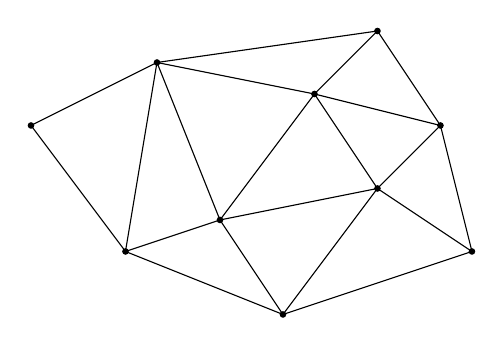
\begin{tikzpicture}[scale=0.4]
		%\draw [<->,thick] (0,10) node (yaxis) [left] {}
		%|- (15,0) node (xaxis) [below] {};
		%centroids
		\fill ( 2, 7) circle (3pt);
		\fill ( 5, 3) circle (3pt);
		\fill ( 6, 9) circle (3pt);
		\fill ( 8, 4) circle (3pt);
		\fill (10, 1) circle (3pt);
		\fill (11, 8) circle (3pt);
		\fill (13, 5) circle (3pt);
		\fill (13,10) circle (3pt);
		\fill (15, 7) circle (3pt);
		\fill (16, 3) circle (3pt);
		
		
		\draw [-] ( 2,7) -- ( 6,9);
		\draw [-] ( 6,9) -- ( 5,3);
		\draw [-] ( 5,3) -- ( 2,7);
		\draw [-] ( 6,9) -- ( 8,4);
		\draw [-] (10,1) -- ( 8,4);
		\draw [-] ( 5,3) -- (10,1);
		\draw [-] ( 8,4) -- ( 5,3);
		\draw [-] ( 8,4) -- (11,8);
		\draw [-] (11,8) -- (6,9);
		\draw [-] ( 6,9) -- (13,10);
		\draw [-] (11,8) -- (13,10);
		\draw [-] (15,7) -- (13,10);
		\draw [-] (16,3) -- (15,7);
		\draw [-] (16,3) -- (10,1);
		\draw [-] (16,3) -- (13,5);
		\draw [-] (13,5) -- (15,7);
		\draw [-] (13,5) -- (10,1);
		\draw [-] (13,5) -- (8,4);
		\draw [-] (13,5) -- (11,8);
		\draw [-] (15,7) -- (11,8);
		\end{tikzpicture}
	\end{center}
	\caption{Example of a Delaunay Triangulation}
	\label{fig:dt1}
\end{figure}
\noindent
More importantly, the Delaunay triangulation of a set of points is the dual graph of its Voronoi Diagram. The edges of the Voronoi diagram, are the line segments connecting the circumcentres of the Delaunay triangles. When overlapped, the duality becomes more obvious. Figure \ref{fig:dt_vd} shows the overlapping of the Voronoi diagram in Figure \ref{fig:vd1} and the Delaunay  triangulation in Figure \ref{fig:dt1}. The Delaunay edges, in black, connect the points at the centre of the Voronoi cells, with edges in blue, to their neighbours.
\begin{figure}[H]
	\begin{center}
		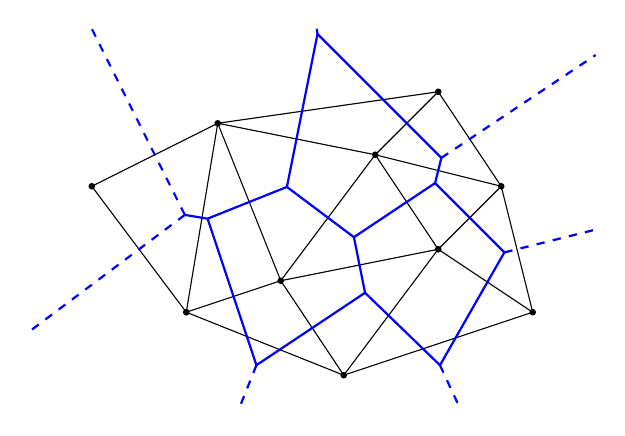
\begin{tikzpicture}[scale=0.4]
		%\draw [<->,thick] (0,10) node (yaxis) [left] {}
		%|- (15,0) node (xaxis) [below] {};
		%centroids
		\fill ( 2, 7) circle (3pt);
		\fill ( 5, 3) circle (3pt);
		\fill ( 6, 9) circle (3pt);
		\fill ( 8, 4) circle (3pt);
		\fill (10, 1) circle (3pt);
		\fill (11, 8) circle (3pt);
		\fill (13, 5) circle (3pt);
		\fill (13,10) circle (3pt);
		\fill (15, 7) circle (3pt);
		\fill (16, 3) circle (3pt);
		
		%DELAUNAY
		\draw [-] ( 2,7) -- ( 6,9);
		\draw [-] ( 6,9) -- ( 5,3);
		\draw [-] ( 5,3) -- ( 2,7);
		\draw [-] ( 6,9) -- ( 8,4);
		\draw [-] (10,1) -- ( 8,4);
		\draw [-] ( 5,3) -- (10,1);
		\draw [-] ( 8,4) -- ( 5,3);
		\draw [-] ( 8,4) -- (11,8);
		\draw [-] (11,8) -- (6,9);
		\draw [-] ( 6,9) -- (13,10);
		\draw [-] (11,8) -- (13,10);
		\draw [-] (15,7) -- (13,10);
		\draw [-] (16,3) -- (15,7);
		\draw [-] (16,3) -- (10,1);
		\draw [-] (16,3) -- (13,5);
		\draw [-] (13,5) -- (15,7);
		\draw [-] (13,5) -- (10,1);
		\draw [-] (13,5) -- (8,4);
		\draw [-] (13,5) -- (11,8);
		\draw [-] (15,7) -- (11,8);
		
		%VORONOI		
		\draw [-,blue,thick] ( 5.6764, 5.9706) -- ( 4.9545, 6.0909);
		\draw [-,blue,thick] ( 5.6764, 5.9706) -- ( 8.1956, 6.9783);
		\draw [-,blue,thick] (10.3235, 5.3824) -- ( 8.1956, 6.9783);
		\draw [-,blue,thick] (10.3235, 5.3824) -- (10.6765, 3.6176);
		\draw [-,blue,thick] ( 7.2272, 1.3182) -- (10.6765, 3.6176);
		\draw [-,blue,thick] ( 7.2272, 1.3182) -- ( 5.6764, 5.9706);
		\draw [-,blue,thick] (13.0556, 1.3182) -- (10.6765, 3.6176);
		\draw [-,blue,thick] (13.0556, 1.3182) -- (15.1000, 4.9000);
		\draw [-,blue,thick] (12.9000, 7.1000) -- (15.1000, 4.9000);
		\draw [-,blue,thick] (12.9000, 7.1000) -- (10.3235, 5.3824);
		\draw [-,blue,thick] (12.9000, 7.1000) -- (13.1000, 7.9000);
		\draw [-,blue,thick] ( 9.1667,11.8333) -- (13.1000, 7.9000);
		\draw [-,blue,thick] ( 9.1667,11.8333) -- ( 8.1956, 6.9783);
		
		\draw [-,blue,thick,dashed] ( 4.9545, 6.0909) -- (	2.0000,12.0000);
		\draw [-,blue,thick,dashed] ( 4.9545, 6.0909) -- (	0.0000,	2.3750);
		\draw [-,blue,thick,dashed] ( 7.2272, 1.3182) -- (	6.7000, 0.0000);
		\draw [-,blue,thick,dashed] (13.0556, 1.3182) -- (13.6667, 0.0000);
		\draw [-,blue,thick,dashed] (15.1000, 4.9000) -- (18.0000, 5.6250);
		\draw [-,blue,thick,dashed] (13.1000, 7.9000) -- (18.0000,11.1667);
		\draw [-,blue,thick,dashed] ( 9.1667,11.8333) -- ( 9.1429,12.0000);
		
		\end{tikzpicture}
	\end{center}
	\caption{Overlap of a Voronoi Diagram and its Delaunay Triangulation}
	\label{fig:dt_vd}
\end{figure}
\noindent
Unlike its counterpart, the Delaunay is much simpler to build incrementally. It is also easier to work with, whilst still providing most of the Voronoi diagram's properties, including the ability to calculate both point location and nearest neighbour searches.
\subsubsection*{Construction}
\label{sect:dtconst}

There are many algorithms to construct a Delaunay triangulation. 
The particular conditions of our approach to the coverage problem impose some restrictions to the choice of the algorithm to use.
Building a Delaunay triangulation can be done incrementally. Starting with a valid triangulation, points can be added, creating and updating existing triangles. An efficient way to do so is to use the Bowyer-Watson algorithm \cite{bwalgo}.

Starting with a valid Delaunay triangulation $\mathcal{T}$, we find the triangle $t$ with vertices $a$,$b$ and $c$ that contains the vertex to insert $v$ using a point location algorithm, such as the line walking algorithm described in the previous section. We then follow algorithm \ref{alg:bowyer} for each vertex $v$ to be included in the triangulation:
\begin{algorithm}[H]
    \caption{Bowyer-Watson Algorithm}
    \begin{algorithmic}[1]
        \Procedure {InsertVertex}{$v,a,b,c$}
            \State $\text{DeleteTriangle}(a,b,c)$
            \State $\text{DigCavity}(v,a,b)$
            \State $\text{DigCavity}(v,b,c)$
            \State $\text{DigCavity}(v,c,a)$
        \EndProcedure
    \end{algorithmic}
    
    \begin{algorithmic}[1]
       	\Procedure {DigCavity}{$a,b,c$}
        	\State $d \gets \text{Adjacent}(b,c)$
        	\If {$d \neq \varnothing$}
	        	\If {$\text{inCircle}(a,b,c,d)$}
		        	\State $\text{DeleteTriangle}(w,v,x)$
		        	\State $\text{DigCavity}(a,b,d)$
		        	\State $\text{DigCavity}(a,d,c)$
	        	\Else 
		        	\State$\text{AddTriangle}(a,b,c)$
	        	\EndIf
        	\EndIf
       	\EndProcedure
    \end{algorithmic}
    \label{alg:bowyer}
\end{algorithm}

The algorithm starts by removing the triangle $t$ that contains the new vertex $v$, and recursively checks adjacent triangles whose circumcircle contains $v$ using the \emph{DigCavity} function. Any triangle that contains $v$ in its circumcircle (calculated with the \emph{InCircle} function), violates the Delaunay rule, and must also be deleted and have its sides recursively checked, until no adjacent triangles violate the Delaunay rule. Whenever the \emph{DigCavity} function reaches a set of three points whose circumcircle does not contain $v$, it creates the triangle by creating counter-clockwise half-edges between those three points (\emph{AddTriangle}). For inserting $n$ points, this algorithm has an expected time complexity of $\bigo(n \log n)$ and is described in more detail by \citet{tricomplex}.

\subsubsection*{Deconstruction}
Deconstructing a Delaunay triangulation usually consists of reversing the construction algorithm to remove points from the triangulation. However, as we will explain in a later chapter, in our case the deconstruction has to be incremental. Since the first point to be removed from the triangulation is necessarily the last one to be inserted, we can use a simpler approach. 
At each step of the construction, all created and removed edges and triangle from the triangulation can be stored in a LIFO structure, or a stack. When the last inserted point is to be removed, recreating the previous state of the triangulation is only a matter of rolling back and retrieving the information from the stack. This also means no geometrical calculations have to be performed, and the old edges and triangles are quickly put back in place, with no new memory allocation needed.

\subsubsection*{Half-Edge Structure}
A useful structure to use when building and managing triangulation meshes is the half-edge structure. The half-edge structure represents one orientation of each edge in the triangulation. This means that for each pair of points ($p_i,p_j$)connected in a triangulation $\mathcal{T}$, there are two directed half-edges: one represents the edge from $p_i$ to $p_j$, and the other represents the opposite direction, connecting $p_j$ to $p_i$. They both contain information about the triangle that they face, and thus, are part of. Triangles are defined by three half edges. All the half edges in the triangle share two of the vertices of the triangle, and are all sorted in a counter-clockwise order. 
Figure \ref{fig:hedge} further illustrates the concept of the half-edges.\\
\begin{figure}[!h]
	\begin{center}
		\begin{tikzpicture}[scale=0.9,
		arr/.style={->,>=stealth',thick,black,shorten >=3pt,shorten <=3pt},
		edg/.style={black,shorten >=6pt,shorten <=6pt},
		par/.style={decoration={sl,raise=2pt},decorate}]
		
		\node [fill,circle,inner sep=3pt,label=below right:$a$] (A) at (6,1){};
		\node [fill,circle,inner sep=3pt,label=above: $b$] (B) at (5,5){};
		\node [fill,circle,inner sep=3pt,label=left: $c$] (C) at (1,2){};
		\node [fill,circle,inner sep=3pt,label=above right:$d$] (D) at (9,6){};
		
		\path[->,>=latex]
		(A) edge [arr,par](B)
		(B) edge [arr,par](C)
		(C) edge [arr,par](B)
		(C) edge [arr,par](A)
		(A) edge [arr,par](C)
		
		(B) edge [arr,par](A)
		(A) edge [arr,par](D)
		(D) edge [arr,par](B)
		(D) edge [arr,par](A)
		(B) edge [arr,par](D);
		\draw [arr,par,dashed,gray] (B) -- (3,7);
		\draw [arr,par,dashed,gray] (3,7) -- (B);
		
		\draw [arr,par,dashed,gray] (C) -- (0.5,0);
		\draw [arr,par,dashed,gray] (0.5,0) -- (C);
		
		\draw [arr,par,dashed,gray] (C) -- (0,4);
		\draw [arr,par,dashed,gray] (0,4) -- (C);
		
		\draw [arr,par,dashed,gray] (A) -- (5,0);
		\draw [arr,par,dashed,gray] (5,0) -- (A);
		
		\draw [arr,par,dashed,gray] (A) -- (10,2);
		\draw [arr,par,dashed,gray] (10,2) -- (A);
		
		\draw [arr,par,dashed,gray] (D) -- (10,4);
		\draw [arr,par,dashed,gray] (10,4) -- (D);
		
		\draw [arr,par,dashed,gray] (D) -- (7,7);
		\draw [arr,par,dashed,gray] (7,7) -- (D);

		
%		\path[-,color=gray]
%		(A) edge (B)
%		(B) edge (C)
%		(C) edge (A)
%		(A) edge (D)
%		(D) edge (B)		
%		;
		\end{tikzpicture}
	\end{center}
	\caption{Illustration of the Half-Edge Structure}
	\label{fig:hedge}
\end{figure}
This structure makes it easier to store the changes to the triangulation at each step, since they contain the information about the triangles themselves. This means that only the half edges need to be stored in the stack (for construction and deconstruction) with no need to manage the triangles directly.
The half-edge structure helps to obtain the triangulation neighbours for any vertex $v$, since it keeps all the edges starting at any given point easily accessible. All neighbours to any point $v$ are the end points to the half-edges starting at $v$. This property is useful when efficiently implementing the greedy routing algorithm described in the following Section. 

\subsubsection*{Greedy Routing}
\label{r:gr}
In order to quickly calculate the nearest neighbour to a point in a set, one can make use of the Delaunay triangulation with Greedy Routing \cite{greedyroute}.
Consider a triangulation $\mathcal{T}$. In order to find the closest vertex in $\mathcal{T}$ to a new point $p$, start at an arbitrary vertex of $\mathcal{T}$, $v$, and find a neighbour $u$ of $v$ whose distance to $p$ is smaller than the distance between $p$ and $v$. Repeat the process for $u$ and its neighbours. When a point $w$ is reached such that no neighbours of $w$ are closer to $p$ than $w$ is, the closest point to $p$ in $\mathcal{T}$ has been found. In the following, we show that the greedy routing algorithm is correct:
\begin{figure}[H]
	\begin{center}
		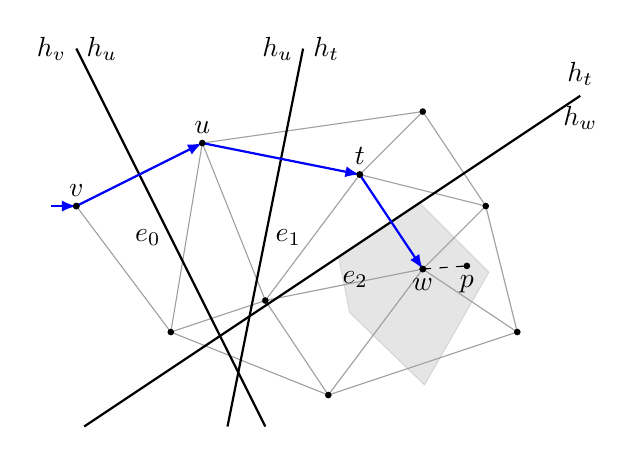
\begin{tikzpicture}[scale=0.4]
		%\draw [<->,thick] (0,10) node (yaxis) [left] {}
		%|- (15,0) node (xaxis) [below] {};
		
		%VORONOI
%		\draw [-,gray!50] ( 5.6764, 5.9706) -- ( 4.9545, 6.0909);
%		\draw [-,gray!50] ( 5.6764, 5.9706) -- ( 8.1956, 6.9783);
%		\draw [-,gray!50] (10.3235, 5.3824) -- ( 8.1956, 6.9783);
%		\draw [-,gray!50] (10.3235, 5.3824) -- (10.6765, 3.6176);
%		\draw [-,gray!50] ( 7.2272, 1.3182) -- (10.6765, 3.6176);
%		\draw [-,gray!50] ( 7.2272, 1.3182) -- ( 5.6764, 5.9706);
%		\draw [-,gray!50] (13.0556, 1.3182) -- (10.6765, 3.6176);
%		\draw [-,gray!50] (13.0556, 1.3182) -- (15.1000, 4.9000);
%		\draw [-,gray!50] (12.9000, 7.1000) -- (15.1000, 4.9000);
%		\draw [-,gray!50] (12.9000, 7.1000) -- (10.3235, 5.3824);
%		\draw [-,gray!50] (12.9000, 7.1000) -- (13.1000, 7.9000);
%		\draw [-,gray!50] ( 9.1667,11.8333) -- (13.1000, 7.9000);
%		%\draw [-,gray!50] ( 9.1667,11.8333) -- ( 8.1956, 6.9783);
%		%VORONOI EXTENDED
%		\draw [-,gray!50] ( 4.9545, 6.0909) -- (2 , 12);
%		\draw [-,gray!50] ( 4.9545, 6.0909) -- (0, 2.375);
%		\draw [-,gray!50] ( 7.2272, 1.3182) -- ( 6.7, 0);
%		\draw [-,gray!50] (13.0556, 1.3182) -- (13.6667, 0);
%		\draw [-,gray!50] (15.1000, 4.9000) -- (18, 5.625);
%		\draw [-,gray!50] (13.1000, 7.9000) -- (18, 11.1667);
%		\draw [-,gray!50] ( 9.1667,11.8333) -- ( 9.1429, 12);
		
		\filldraw[fill=black, opacity=0.1] 	(10.3235, 5.3824) -- (10.6765, 3.6176) --
											(13.0556, 1.3182) -- (15.1000, 4.9000) --
											(12.9000, 7.1000) -- cycle;
		
		%DELAUNAY
		\draw [-,gray!75] ( 2,7) -- ( 6,9);
		\draw [-,gray!75] ( 6,9) -- ( 5,3);
		\draw [-,gray!75] ( 5,3) -- ( 2,7);
		\draw [-,gray!75] ( 6,9) -- ( 8,4);
		\draw [-,gray!75] (10,1) -- ( 8,4);
		\draw [-,gray!75] ( 5,3) -- (10,1);
		\draw [-,gray!75] ( 8,4) -- ( 5,3);
		\draw [-,gray!75] ( 8,4) -- (11,8);
		\draw [-,gray!75] (11,8) -- (6,9);
		\draw [-,gray!75] ( 6,9) -- (13,10);
		\draw [-,gray!75] (11,8) -- (13,10);
		\draw [-,gray!75] (15,7) -- (13,10);
		\draw [-,gray!75] (16,3) -- (15,7);
		\draw [-,gray!75] (16,3) -- (10,1);
		\draw [-,gray!75] (16,3) -- (13,5);
		\draw [-,gray!75] (13,5) -- (15,7);
		\draw [-,gray!75] (13,5) -- (10,1);
		\draw [-,gray!75] (13,5) -- (8,4);
		\draw [-,gray!75] (13,5) -- (11,8);
		\draw [-,gray!75] (15,7) -- (11,8);
		
		
		%POINTS
		
		\fill ( 2, 7) circle (3pt);
		\fill ( 5, 3) circle (3pt);
		\fill ( 8, 4) circle (3pt);
		\fill (10, 1) circle (3pt);
		\fill (11, 8) circle (3pt);
		\fill (13, 5) circle (3pt);
		\fill (13,10) circle (3pt);
		\fill (15, 7) circle (3pt);
		\fill (16, 3) circle (3pt);
		
		%EDGE E
		\draw [-,thick] ( 8,0)		-- node[left]{$e_0$} ( 2, 12)	node[left]		{$h_v$} node[right]{$h_u$};
		\draw [-,thick] ( 6.8,0)	-- node[right]{$e_1$} (9.2,12)	node[left] 		{$h_u$} node[right]{$h_t$};
		\draw [-,thick] ( 2.25,0)	-- node[below right]{$e_2$} (18,10.5)	node[above]{$h_t$} node[below]{$h_w$};
		
		
		\draw [-,dashed]( 13,5) -- ( 14.4, 5.1);
		\draw [->,>=latex,thick,blue]( 1.2,7) -- (  2,7);
		\draw [->,>=latex,thick,blue]( 2,7) -- (  6,9);
		\draw [->,>=latex,thick,blue]( 6,9) -- ( 11, 8);
		\draw [->,>=latex,thick,blue](11,8) -- ( 13, 5);
		\fill (14.4, 5.1) circle (3pt) node[anchor=north]{$p$};
		\fill ( 2, 7)     circle (3pt) node[anchor=south]{$v$};
		\fill ( 6, 9)     circle (3pt) node[anchor=south]{$u$};
		\fill (11, 8)     circle (3pt) node[anchor=south]{$t$};
		\fill (13, 5)     circle (3pt) node[anchor=north]{$w$};
		
		\end{tikzpicture}
	\end{center}
\end{figure}
\noindent
In Figure \ref{fig:gr1}, the search for the closest vertex to $p$ starts at point $v$. From there, point $u$, which is closer to $p$ than $v$ is, is found. The step is repeated, following the blue path until point $w$ is reached. Since no neighbour of $w$ is closer to $p$ than $w$ is, then $p$ must be within the Voronoi cell of point $w$ (shaded light grey).
\begin{theorem}
\cite{greedyroute}
There is no point set whose Delaunay triangulation defeats the greedy routing algorithm.
\begin{proof}
For every vertex $v$ in a triangulation $\mathcal{T}$, let the perpendicular bisector of the line segment defined by $v$ and any neighbour $u$ be called $e$ if there is at least one neighbour of $v$, $u$ closer to $p$ than $v$ is. The line $e$ intersects the line segment $(v,p)$ and divides the plane in two open half planes: $h_v$ and $h_u$. Note that the half plane $h_u$ contains $p$. Delaunay edges connect the Voronoi neighbours and their bisectors define the edges of the Voronoi cells, which are convex polygons. Repeating the process recursively for $u$, if a point $w$ is found, whose neighbourhood contains no points closer to $p$ than itself, then $p$ is contained within all possible open half planes containing $w$, defined by $w$ and all its neighbours. Point $p$ is then by definition located in point $w$'s Voronoi cell. This means that $w$ is the point in $\mathcal{T}$ closest to $p$.
\end{proof}
\end{theorem}
\subsubsection*{Line Walking}
Another point location algorithm to consider is the line walking algorithm \cite{walking}. This algorithm finds a triangle $t$ in a triangulation $\mathcal{T}$ that contains a given point $v$. 
Starting at any triangle $s$, with the geometrical centre $m$, if point $v$ is not contained in $s$, then the line segment $(v,m)$ intersects a finite set of triangles.  
The line segment $(v,m)$ intersects two edges of each triangle in this set, with the exception of $s$ and $t$ where $(v,m)$ only intersects one edge each. 
By iterating through each triangle choosing the neighbour triangle that contains the next edge that intersects $(v,m)$, triangle $t$ can be found in $\bigo(n)$ time.

This algorithm was described by \citet{walking}, and is illustrated in the following figure, where the dark shaded triangles represent the starting and finishing triangles, and the light shaded triangles the path the algorithm takes to find the final triangle that contains the vertex $v$.
\begin{figure}[H]
	\begin{center}
		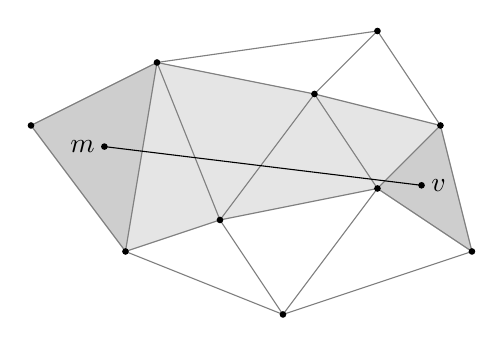
\begin{tikzpicture}[scale=0.4]
		%\draw [<->,thick] (0,10) node (yaxis) [left] {}
		%|- (15,0) node (xaxis) [below] {};
		
		\filldraw[fill=black, opacity=0.1] 	(2,7) -- (6,9) -- 
											(11,8) -- (15,7) -- 
											(16,3) -- (13,5) --
											(8,4) -- (5,3) --
											cycle;
		
		\filldraw[fill=black, opacity=0.1] 	(2,7) -- (6,9) -- (5,3) --
											cycle;
											
		\filldraw[fill=black, opacity=0.1] 	(15,7) -- (13,5) -- (16,3) --
													cycle;
		
		
		
		\draw [-,gray] ( 2,7) -- ( 6,9);
		\draw [-,gray] ( 6,9) -- ( 5,3);
		\draw [-,gray] ( 5,3) -- ( 2,7);
		\draw [-,gray] ( 6,9) -- ( 8,4);
		\draw [-,gray] (10,1) -- ( 8,4);
		\draw [-,gray] ( 5,3) -- (10,1);
		\draw [-,gray] ( 8,4) -- ( 5,3);
		\draw [-,gray] ( 8,4) -- (11,8);
		\draw [-,gray] (11,8) -- (6,9);
		\draw [-,gray] ( 6,9) -- (13,10);
		\draw [-,gray] (11,8) -- (13,10);
		\draw [-,gray] (15,7) -- (13,10);
		\draw [-,gray] (16,3) -- (15,7);
		\draw [-,gray] (16,3) -- (10,1);
		\draw [-,gray] (16,3) -- (13,5);
		\draw [-,gray] (13,5) -- (15,7);
		\draw [-,gray] (13,5) -- (10,1);
		\draw [-,gray] (13,5) -- (8,4);
		\draw [-,gray] (13,5) -- (11,8);
		\draw [-,gray] (15,7) -- (11,8);
		
		
		%centroids
		\fill ( 2, 7) circle (3pt);
		\fill ( 5, 3) circle (3pt);
		\fill ( 6, 9) circle (3pt);
		\fill ( 8, 4) circle (3pt);
		\fill (10, 1) circle (3pt);
		\fill (11, 8) circle (3pt);
		\fill (13, 5) circle (3pt);
		\fill (13,10) circle (3pt);
		\fill (15, 7) circle (3pt);
		\fill (16, 3) circle (3pt);
		
		
		\draw [-]( 4.33,6.33) -- ( 14.4, 5.1);
		%\draw []( 2,7) -- node[anchor=south]{$t$} ( 6,9);
		\fill ( 4.33,6.33) circle (3pt) node[anchor=east]{$m$};
		\fill (14.4, 5.1) circle (3pt) node[anchor=west]{$v$};
		\end{tikzpicture}
	\end{center}
	\caption{Illustration of the Walking Algorithm}
	\label{fig:wk1}
\end{figure}
After finding this triangle, the Bowyer-Watson algorithm described in Section \ref{sect:dtconst} can be used to update the new triangulation, which now includes $v$.
\subsection{Hilbert Curves}

Most of the point location algorithms aforementioned have linear time complexity, and most of the worst case scenarios include searching across the plane. These occur when the starting search position is random and does not make use of the spatial organisation of the data. In order to fully take advantage of these approaches, the points should be sorted is such a way that the distance between consecutive points is minimised.

Hilbert curves are a kind of fractal space-filling curves \cite{sfcurves} that generally minimize the Euclidean distance between points close on the curve.

True Hilbert curves map a 2-dimensional space in a 1-dimension line. This line has an infinite length, which makes mapping 2-dimensional points to it infeasible. Instead, discrete approximations are used. Since the true curve is fractal, the approximations are defined by the number of fractal steps it takes in order to reach them. Figure \ref*{fig:hilbert} demonstrates the first few orders of approximation:
\begin{figure}[H]
	\begin{center}
		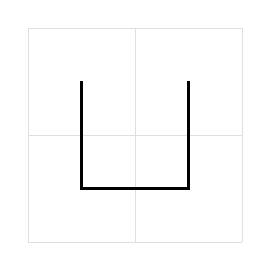
\begin{tikzpicture}[scale=0.17]
		\draw [step=8,gray,very thin,opacity=0.25](0,0) grid(16,16);
		\draw [-,thick] 	(4,12) -- ( 4,4) -- ( 12,4) -- ( 12,12);
		\end{tikzpicture}
		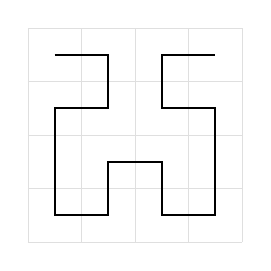
\begin{tikzpicture}[scale=0.17]
		\draw [step=4,gray,very thin,opacity=0.25](0,0) grid(16,16);
		\draw [-,thick]
				 	(2,14) -- ( 6,14) -- (6,10) -- (2,10) -- 
					(2,2)  -- (6,2) -- (6,6) -- (10,6) -- 
					(10,2) -- (14,2) -- (14,10)--(10,10) --
					(10,14) -- (14,14);
		\end{tikzpicture}
		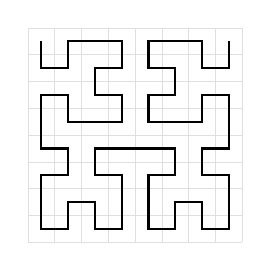
\begin{tikzpicture}[scale=0.17]
		\draw [step=2,gray,very thin,opacity=0.25](0,0) grid(16,16);
		\draw [-,thick] 
					(1,15) 	-- (1,13) 	-- (3,13) 	-- (3,15) 	-- (7,15) 	--
					(7,13) 	-- (5,13) 	-- (5,11)	-- (7,11) 	-- (7,9) 	--
					(3,9) 	-- (3,11)	-- (1,11)	-- (1,7) 	-- (3,7) 	--
					(3,5) 	-- (1,5) 	-- (1,1)	-- (3,1) 	-- (3,3) 	-- 
					(5,3) 	-- (5,1) 	-- (7,1)  	-- (7,5) 	-- (5,5) 	--
					(5,7) 	-- (11,7) 	-- (11,5)  	-- (9,5) 	-- (9,1) 	--
					(11,1)	-- (11,3) 	-- (13,3)  	-- (13,1) 	-- (15,1) 	--
					(15,5) 	-- (13,5) 	-- (13,7)  	-- (15,7) 	-- (15,11)	--
					(13,11)	-- (13,9)  	-- (9,9) 	-- (9,11) 	-- (11,11)	--
					(11,13)	-- (9,13) 	-- (9,15) 	-- (13,15)  -- (13,13) 	--
					(15,13) -- (15,15)
					;
		
		\end{tikzpicture}
		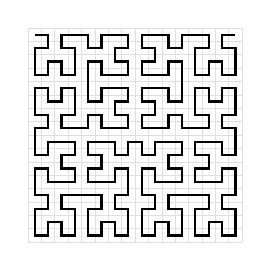
\begin{tikzpicture}[scale=0.17]
		\draw [step=1,gray,very thin,opacity=0.25](0,0) grid(16,16);
		\draw [-,thick] 
				(0.5, 15.5)	-- (1.5, 15.5) 	-- (1.5, 14.5) 	-- (0.5, 14.5) 	-- 
				(0.5, 13.5)	-- (0.5, 12.5) 	-- (1.5, 12.5) 	-- (1.5, 13.5) 	-- 
				(2.5, 13.5)	-- (2.5, 12.5) 	-- (3.5, 12.5) 	-- (3.5, 13.5) 	-- 
				(3.5, 14.5) -- (2.5, 14.5) 	-- (2.5, 15.5) 	-- (3.5, 15.5) 	-- 
				(4.5, 15.5) -- (4.5, 14.5) 	-- (5.5, 14.5) 	-- (5.5, 15.5) 	-- 
				(6.5, 15.5) -- (7.5, 15.5) 	-- (7.5, 14.5) 	-- (6.5, 14.5) 	-- 
				(6.5, 13.5) -- (7.5, 13.5) 	-- (7.5, 12.5) 	-- (6.5, 12.5) 	-- 
				(5.5, 12.5) -- (5.5, 13.5) 	-- (4.5, 13.5) 	-- (4.5, 12.5) 	-- 
				(4.5, 11.5) -- (4.5, 10.5) 	-- (5.5, 10.5) 	-- (5.5, 11.5) 	-- 
				(6.5, 11.5) -- (7.5, 11.5) 	-- (7.5, 10.5) 	-- (6.5, 10.5) 	-- 
				(6.5, 9.5) 	-- (7.5, 9.5) 	-- (7.5, 8.5) 	-- (6.5, 8.5) 	-- 
				(5.5, 8.5) 	-- (5.5, 9.5) 	-- (4.5, 9.5) 	-- (4.5, 8.5) 	-- 
				(3.5, 8.5) 	-- (2.5, 8.5) 	-- (2.5, 9.5) 	-- (3.5, 9.5) 	-- 
				(3.5, 10.5) -- (3.5, 11.5) 	-- (2.5, 11.5) 	-- (2.5, 10.5) 	-- 
				(1.5, 10.5) -- (1.5, 11.5) 	-- (0.5, 11.5) 	-- (0.5, 10.5) 	-- 
				(0.5, 9.5) 	-- (1.5, 9.5)	-- (1.5, 8.5) 	-- (0.5, 8.5) 	-- 
				(0.5, 7.5) 	-- (0.5, 6.5) 	-- (1.5, 6.5) 	-- (1.5, 7.5) 	-- 
				(2.5, 7.5) 	-- (3.5, 7.5) 	-- (3.5, 6.5) 	-- (2.5, 6.5) 	-- 
				(2.5, 5.5) 	-- (3.5, 5.5) 	-- (3.5, 4.5) 	-- (2.5, 4.5) 	-- 
				(1.5, 4.5) 	-- (1.5, 5.5) 	-- (0.5, 5.5) 	-- (0.5, 4.5) 	-- 
				(0.5, 3.5) 	-- (1.5, 3.5) 	-- (1.5, 2.5) 	-- (0.5, 2.5) 	-- 
				(0.5, 1.5) 	-- (0.5, 0.5) 	-- (1.5, 0.5)	-- (1.5, 1.5) 	-- 
				(2.5, 1.5) 	-- (2.5, 0.5) 	-- (3.5, 0.5) 	-- (3.5, 1.5) 	-- 
				(3.5, 2.5) 	-- (2.5, 2.5) 	-- (2.5, 3.5) 	-- (3.5, 3.5) 	-- 
				(4.5, 3.5) 	-- (5.5, 3.5) 	-- (5.5, 2.5) 	-- (4.5, 2.5) 	-- 
				(4.5, 1.5) 	-- (4.5, 0.5) 	-- (5.5, 0.5) 	-- (5.5, 1.5) 	-- 
				(6.5, 1.5) 	-- (6.5, 0.5) 	-- (7.5, 0.5) 	-- (7.5, 1.5) 	-- 
				(7.5, 2.5) 	-- (6.5, 2.5) 	-- (6.5, 3.5) 	-- (7.5, 3.5) 	-- 
				(7.5, 4.5) 	-- (7.5, 5.5) 	-- (6.5, 5.5) 	-- (6.5, 4.5) 	-- 
				(5.5, 4.5) 	-- (4.5, 4.5) 	-- (4.5, 5.5) 	-- (5.5, 5.5) 	-- 
				(5.5, 6.5) 	-- (4.5, 6.5) 	-- (4.5, 7.5) 	-- (5.5, 7.5) 	-- 
				(6.5, 7.5) 	-- (6.5, 6.5) 	-- (7.5, 6.5) 	-- (7.5, 7.5) 	-- 
				(8.5, 7.5) 	-- (8.5, 6.5) 	-- (9.5, 6.5) 	-- (9.5, 7.5) 	-- 
				(10.5, 7.5) -- (11.5, 7.5) 	-- (11.5, 6.5) 	-- (10.5, 6.5) 	-- 
				(10.5, 5.5)	-- (11.5, 5.5) 	-- (11.5, 4.5) 	-- (10.5, 4.5) 	-- 
				(9.5, 4.5) 	-- (9.5, 5.5) 	-- (8.5, 5.5) 	-- (8.5, 4.5) 	-- 
				(8.5, 3.5) 	-- (9.5, 3.5) 	-- (9.5, 2.5) 	-- (8.5, 2.5) 	-- 
				(8.5, 1.5) 	-- (8.5, 0.5) 	-- (9.5, 0.5) 	-- (9.5, 1.5) 	-- 
				(10.5, 1.5) -- (10.5, 0.5) 	-- (11.5, 0.5) 	-- (11.5, 1.5) 	-- 
				(11.5, 2.5) -- (10.5, 2.5) 	-- (10.5, 3.5) 	-- (11.5, 3.5) 	-- 
				(12.5, 3.5) -- (13.5, 3.5)	-- (13.5, 2.5) 	-- (12.5, 2.5) 	-- 
				(12.5, 1.5) -- (12.5, 0.5) 	-- (13.5, 0.5) 	-- (13.5, 1.5) 	-- 
				(14.5, 1.5) -- (14.5, 0.5) 	-- (15.5, 0.5) 	-- (15.5, 1.5) 	-- 
				(15.5, 2.5) -- (14.5, 2.5) 	-- (14.5, 3.5) 	-- (15.5, 3.5) 	-- 
				(15.5, 4.5) -- (15.5, 5.5) 	-- (14.5, 5.5) 	-- (14.5, 4.5) 	-- 
				(13.5, 4.5) -- (12.5, 4.5) 	-- (12.5, 5.5) 	-- (13.5, 5.5) 	-- 
				(13.5, 6.5) -- (12.5, 6.5) 	-- (12.5, 7.5) 	-- (13.5, 7.5) 	-- 
				(14.5, 7.5) -- (14.5, 6.5) 	-- (15.5, 6.5) 	-- (15.5, 7.5) 	-- 
				(15.5, 8.5) -- (14.5, 8.5) 	-- (14.5, 9.5) 	-- (15.5, 9.5) 	-- 
				(15.5, 10.5)-- (15.5, 11.5)	-- (14.5, 11.5)	-- (14.5, 10.5)	-- 
				(13.5, 10.5)-- (13.5, 11.5)	-- (12.5, 11.5)	-- (12.5, 10.5)	--
				(12.5, 9.5)	-- (13.5, 9.5) 	-- (13.5, 8.5)	-- (12.5, 8.5) 	-- 
				(11.5, 8.5) -- (11.5, 9.5) 	-- (10.5, 9.5) 	-- (10.5, 8.5) 	-- 
				(9.5, 8.5) 	-- (8.5, 8.5) 	-- (8.5, 9.5) 	-- (9.5, 9.5) 	--
				(9.5, 10.5) -- (8.5, 10.5) 	-- (8.5, 11.5) 	-- (9.5, 11.5) 	-- 
				(10.5, 11.5)-- (10.5, 10.5)	-- (11.5, 10.5)	-- (11.5, 11.5)	-- 
				(11.5, 12.5)-- (11.5, 13.5)	-- (10.5, 13.5)	-- (10.5, 12.5)	-- 
				(9.5, 12.5) -- (8.5, 12.5) 	-- (8.5, 13.5) 	-- (9.5, 13.5) 	-- 
				(9.5, 14.5) -- (8.5, 14.5) 	-- (8.5, 15.5) 	-- (9.5, 15.5) 	--
				(10.5, 15.5)-- (10.5, 14.5)	-- (11.5, 14.5)	-- (11.5, 15.5)	-- 
				(12.5, 15.5)-- (13.5, 15.5)	-- (13.5, 14.5)	-- (12.5, 14.5)	-- 
				(12.5, 13.5)-- (12.5, 12.5)	-- (13.5, 12.5)	-- (13.5, 13.5)	--
				(14.5, 13.5)-- (14.5, 12.5)	-- (15.5, 12.5)	-- (15.5, 13.5)	--
				(15.5, 14.5)-- (14.5, 14.5)	-- (14.5, 15.5)	-- (15.5, 15.5)
		;		
		\end{tikzpicture}
		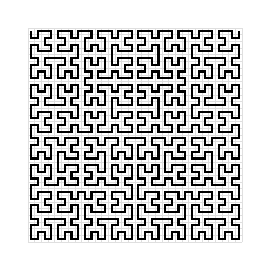
\begin{tikzpicture}[scale=0.17]
		\draw [step=0.5,gray,very thin,opacity=0.25](0,0) grid(16,16);
		\draw [-,thick]
					(15.75,15.75)	--(15.75, 15.25) 	-- (15.25, 15.25) 	-- (15.25, 15.75) 	-- (14.75, 15.75) 	-- (14.25, 15.75) 	-- (14.25, 15.25) 	-- (14.75, 15.25) 	-- (14.75, 14.75) 	-- (14.25, 14.75) 	-- (14.25, 14.25) 	-- (14.75, 14.25) 	-- (15.25, 14.25) 	-- (15.25, 14.75) 	-- (15.75, 14.75) 	-- (15.75, 14.25) 	-- (15.75, 13.75) 	-- (15.25, 13.75) 	-- (15.25, 13.25) 	-- (15.75, 13.25) 	-- (15.75, 12.75) 	-- (15.75, 12.25) 	-- (15.25, 12.25) 	-- (15.25, 12.75) 	-- (14.75, 12.75) 	-- (14.75, 12.25) 	-- (14.25, 12.25) 	-- (14.25, 12.75) 	-- (14.25, 13.25) 	-- (14.75, 13.25) 	-- (14.75, 13.75) 	-- (14.25, 13.75) 	-- (13.75, 13.75) 	-- (13.25, 13.75) 	-- (13.25, 13.25) 	-- (13.75, 13.25) 	-- (13.75, 12.75) 	-- (13.75, 12.25) 	-- (13.25, 12.25) 	-- (13.25, 12.75) 	-- (12.75, 12.75) 	-- (12.75, 12.25) 	-- (12.25, 12.25) 	-- (12.25, 12.75) 	-- (12.25, 13.25) 	-- (12.75, 13.25) 	-- (12.75, 13.75) 	-- (12.25, 13.75) 	-- (12.25, 14.25) 	-- (12.25, 14.75) 	-- (12.75, 14.75) 	-- (12.75, 14.25) 	-- (13.25, 14.25) 	-- (13.75, 14.25) 	-- (13.75, 14.75) 	-- (13.25, 14.75) 	-- (13.25, 15.25) 	-- (13.75, 15.25) 	-- (13.75, 15.75) 	-- (13.25, 15.75) 	-- (12.75, 15.75) 	-- (12.75, 15.25) 	-- (12.25, 15.25) 	-- (12.25, 15.75) 	-- (11.75, 15.75) 	-- (11.25, 15.75) 	-- (11.25, 15.25) 	-- (11.75, 15.25) 	-- (11.75, 14.75) 	-- (11.75, 14.25) 	-- (11.25, 14.25) 	-- (11.25, 14.75) 	-- (10.75, 14.75) 	-- (10.75, 14.25) 	-- (10.25, 14.25) 	-- (10.25, 14.75) 	-- (10.25, 15.25) 	-- (10.75, 15.25) 	-- (10.75, 15.75) 	-- (10.25, 15.75) 	-- (9.75, 15.75) 	-- (9.75, 15.25) 	-- (9.25, 15.25) 	-- (9.25, 15.75) 	-- (8.75, 15.75) 	-- (8.25, 15.75) 	-- (8.25, 15.25) 	-- (8.75, 15.25) 	-- (8.75, 14.75) 	-- (8.25, 14.75) 	-- (8.25, 14.25) 	-- (8.75, 14.25) 	-- (9.25, 14.25) 	-- (9.25, 14.75) 	-- (9.75, 14.75) 	-- (9.75, 14.25) 	-- (9.75, 13.75) 	-- (9.75, 13.25) 	-- (9.25, 13.25) 	-- (9.25, 13.75) 	-- (8.75, 13.75) 	-- (8.25, 13.75) 	-- (8.25, 13.25) 	-- (8.75, 13.25) 	-- (8.75, 12.75) 	-- (8.25, 12.75) 	-- (8.25, 12.25) 	-- (8.75, 12.25) 	-- (9.25, 12.25) 	-- (9.25, 12.75) 	-- (9.75, 12.75) 	-- (9.75, 12.25) 	-- (10.25, 12.25) 	-- (10.75, 12.25) 	-- (10.75, 12.75) 	-- (10.25, 12.75) 	-- (10.25, 13.25) 	-- (10.25, 13.75) 	-- (10.75, 13.75) 	-- (10.75, 13.25) 	-- (11.25, 13.25) 	-- (11.25, 13.75) 	-- (11.75, 13.75) 	-- (11.75, 13.25) 	-- (11.75, 12.75) 	-- (11.25, 12.75) 	-- (11.25, 12.25) 	-- (11.75, 12.25) 	-- (11.75, 11.75) 	-- (11.25, 11.75) 	-- (11.25, 11.25) 	-- (11.75, 11.25) 	-- (11.75, 10.75) 	-- (11.75, 10.25) 	-- (11.25, 10.25) 	-- (11.25, 10.75) 	-- (10.75, 10.75) 	-- (10.75, 10.25) 	-- (10.25, 10.25) 	-- (10.25, 10.75) 	-- (10.25, 11.25) 	-- (10.75, 11.25) 	-- (10.75, 11.75) 	-- (10.25, 11.75) 	-- (9.75, 11.75) 	-- (9.75, 11.25) 	-- (9.25, 11.25) 	-- (9.25, 11.75) 	-- (8.75, 11.75) 	-- (8.25, 11.75) 	-- (8.25, 11.25) 	-- (8.75, 11.25) 	-- (8.75, 10.75) 	-- (8.25, 10.75) 	-- (8.25, 10.25) 	-- (8.75, 10.25) 	-- (9.25, 10.25) 	-- (9.25, 10.75) 	-- (9.75, 10.75) 	-- (9.75, 10.25) 	-- (9.75, 9.75) 	-- (9.75, 9.25) 	-- (9.25, 9.25) 	-- (9.25, 9.75) 	-- (8.75, 9.75) 	-- (8.25, 9.75) 	-- (8.25, 9.25) 	-- (8.75, 9.25) 	-- (8.75, 8.75) 	-- (8.25, 8.75) 	-- (8.25, 8.25) 	-- (8.75, 8.25) 	-- (9.25, 8.25) 	-- (9.25, 8.75) 	-- (9.75, 8.75) 	-- (9.75, 8.25) 	-- (10.25, 8.25) 	-- (10.75, 8.25) 	-- (10.75, 8.75) 	-- (10.25, 8.75) 	-- (10.25, 9.25) 	-- (10.25, 9.75) 	-- (10.75, 9.75) 	-- (10.75, 9.25) 	-- (11.25, 9.25) 	-- (11.25, 9.75) 	-- (11.75, 9.75) 	-- (11.75, 9.25) 	-- (11.75, 8.75) 	-- (11.25, 8.75) 	-- (11.25, 8.25) 	-- (11.75, 8.25) 	-- (12.25, 8.25) 	-- (12.25, 8.75) 	-- (12.75, 8.75) 	-- (12.75, 8.25) 	-- (13.25, 8.25) 	-- (13.75, 8.25) 	-- (13.75, 8.75) 	-- (13.25, 8.75) 	-- (13.25, 9.25) 	-- (13.75, 9.25) 	-- (13.75, 9.75) 	-- (13.25, 9.75) 	-- (12.75, 9.75) 	-- (12.75, 9.25) 	-- (12.25, 9.25) 	-- (12.25, 9.75) 	-- (12.25, 10.25) 	-- (12.75, 10.25) 	-- (12.75, 10.75) 	-- (12.25, 10.75) 	-- (12.25, 11.25) 	-- (12.25, 11.75) 	-- (12.75, 11.75) 	-- (12.75, 11.25) 	-- (13.25, 11.25) 	-- (13.25, 11.75) 	-- (13.75, 11.75) 	-- (13.75, 11.25) 	-- (13.75, 10.75) 	-- (13.25, 10.75) 	-- (13.25, 10.25) 	-- (13.75, 10.25) 	-- (14.25, 10.25) 	-- (14.75, 10.25) 	-- (14.75, 10.75) 	-- (14.25, 10.75) 	-- (14.25, 11.25) 	-- (14.25, 11.75) 	-- (14.75, 11.75) 	-- (14.75, 11.25) 	-- (15.25, 11.25) 	-- (15.25, 11.75) 	-- (15.75, 11.75) 	-- (15.75, 11.25) 	-- (15.75, 10.75) 	-- (15.25, 10.75) 	-- (15.25, 10.25) 	-- (15.75, 10.25) 	-- (15.75, 9.75) 	-- (15.75, 9.25) 	-- (15.25, 9.25) 	-- (15.25, 9.75) 	-- (14.75, 9.75) 	-- (14.25, 9.75) 	-- (14.25, 9.25) 	-- (14.75, 9.25) 	-- (14.75, 8.75) 	-- (14.25, 8.75) 	-- (14.25, 8.25) 	-- (14.75, 8.25) 	-- (15.25, 8.25) 	-- (15.25, 8.75) 	-- (15.75, 8.75) 	-- (15.75, 8.25) 	-- (15.75, 7.75) 	-- (15.25, 7.75) 	-- (15.25, 7.25) 	-- (15.75, 7.25) 	-- (15.75, 6.75) 	-- (15.75, 6.25) 	-- (15.25, 6.25) 	-- (15.25, 6.75) 	-- (14.75, 6.75) 	-- (14.75, 6.25) 	-- (14.25, 6.25) 	-- (14.25, 6.75) 	-- (14.25, 7.25) 	-- (14.75, 7.25) 	-- (14.75, 7.75) 	-- (14.25, 7.75) 	-- (13.75, 7.75) 	-- (13.75, 7.25) 	-- (13.25, 7.25) 	-- (13.25, 7.75) 	-- (12.75, 7.75) 	-- (12.25, 7.75) 	-- (12.25, 7.25) 	-- (12.75, 7.25) 	-- (12.75, 6.75) 	-- (12.25, 6.75) 	-- (12.25, 6.25) 	-- (12.75, 6.25) 	-- (13.25, 6.25) 	-- (13.25, 6.75) 	-- (13.75, 6.75) 	-- (13.75, 6.25) 	-- (13.75, 5.75) 	-- (13.75, 5.25) 	-- (13.25, 5.25) 	-- (13.25, 5.75) 	-- (12.75, 5.75) 	-- (12.25, 5.75) 	-- (12.25, 5.25) 	-- (12.75, 5.25) 	-- (12.75, 4.75) 	-- (12.25, 4.75) 	-- (12.25, 4.25) 	-- (12.75, 4.25) 	-- (13.25, 4.25) 	-- (13.25, 4.75) 	-- (13.75, 4.75) 	-- (13.75, 4.25) 	-- (14.25, 4.25) 	-- (14.75, 4.25) 	-- (14.75, 4.75) 	-- (14.25, 4.75) 	-- (14.25, 5.25) 	-- (14.25, 5.75) 	-- (14.75, 5.75) 	-- (14.75, 5.25) 	-- (15.25, 5.25) 	-- (15.25, 5.75) 	-- (15.75, 5.75) 	-- (15.75, 5.25) 	-- (15.75, 4.75) 	-- (15.25, 4.75) 	-- (15.25, 4.25) 	-- (15.75, 4.25) 	-- (15.75, 3.75) 	-- (15.75, 3.25) 	-- (15.25, 3.25) 	-- (15.25, 3.75) 	-- (14.75, 3.75) 	-- (14.25, 3.75) 	-- (14.25, 3.25) 	-- (14.75, 3.25) 	-- (14.75, 2.75) 	-- (14.25, 2.75) 	-- (14.25, 2.25) 	-- (14.75, 2.25) 	-- (15.25, 2.25) 	-- (15.25, 2.75) 	-- (15.75, 2.75) 	-- (15.75, 2.25) 	-- (15.75, 1.75) 	-- (15.25, 1.75) 	-- (15.25, 1.25) 	-- (15.75, 1.25) 	-- (15.75, 0.75) 	-- (15.75, 0.25) 	-- (15.25, 0.25) 	-- (15.25, 0.75) 	-- (14.75, 0.75) 	-- (14.75, 0.25) 	-- (14.25, 0.25) 	-- (14.25, 0.75) 	-- (14.25, 1.25) 	-- (14.75, 1.25) 	-- (14.75, 1.75) 	-- (14.25, 1.75) 	-- (13.75, 1.75) 	-- (13.25, 1.75) 	-- (13.25, 1.25) 	-- (13.75, 1.25) 	-- (13.75, 0.75) 	-- (13.75, 0.25) 	-- (13.25, 0.25) 	-- (13.25, 0.75) 	-- (12.75, 0.75) 	-- (12.75, 0.25) 	-- (12.25, 0.25) 	-- (12.25, 0.75) 	-- (12.25, 1.25) 	-- (12.75, 1.25) 	-- (12.75, 1.75) 	-- (12.25, 1.75) 	-- (12.25, 2.25) 	-- (12.25, 2.75) 	-- (12.75, 2.75) 	-- (12.75, 2.25) 	-- (13.25, 2.25) 	-- (13.75, 2.25) 	-- (13.75, 2.75) 	-- (13.25, 2.75) 	-- (13.25, 3.25) 	-- (13.75, 3.25) 	-- (13.75, 3.75) 	-- (13.25, 3.75) 	-- (12.75, 3.75) 	-- (12.75, 3.25) 	-- (12.25, 3.25) 	-- (12.25, 3.75) 	-- (11.75, 3.75) 	-- (11.75, 3.25) 	-- (11.25, 3.25) 	-- (11.25, 3.75) 	-- (10.75, 3.75) 	-- (10.25, 3.75) 	-- (10.25, 3.25) 	-- (10.75, 3.25) 	-- (10.75, 2.75) 	-- (10.25, 2.75) 	-- (10.25, 2.25) 	-- (10.75, 2.25) 	-- (11.25, 2.25) 	-- (11.25, 2.75) 	-- (11.75, 2.75) 	-- (11.75, 2.25) 	-- (11.75, 1.75) 	-- (11.25, 1.75) 	-- (11.25, 1.25) 	-- (11.75, 1.25) 	-- (11.75, 0.75) 	-- (11.75, 0.25) 	-- (11.25, 0.25) 	-- (11.25, 0.75) 	-- (10.75, 0.75) 	-- (10.75, 0.25) 	-- (10.25, 0.25) 	-- (10.25, 0.75) 	-- (10.25, 1.25) 	-- (10.75, 1.25) 	-- (10.75, 1.75) 	-- (10.25, 1.75) 	-- (9.75, 1.75) 	-- (9.25, 1.75) 	-- (9.25, 1.25) 	-- (9.75, 1.25) 	-- (9.75, 0.75) 	-- (9.75, 0.25) 	-- (9.25, 0.25) 	-- (9.25, 0.75) 	-- (8.75, 0.75) 	-- (8.75, 0.25) 	-- (8.25, 0.25) 	-- (8.25, 0.75) 	-- (8.25, 1.25) 	-- (8.75, 1.25) 	-- (8.75, 1.75) 	-- (8.25, 1.75) 	-- (8.25, 2.25) 	-- (8.25, 2.75) 	-- (8.75, 2.75) 	-- (8.75, 2.25) 	-- (9.25, 2.25) 	-- (9.75, 2.25) 	-- (9.75, 2.75) 	-- (9.25, 2.75) 	-- (9.25, 3.25) 	-- (9.75, 3.25) 	-- (9.75, 3.75) 	-- (9.25, 3.75) 	-- (8.75, 3.75) 	-- (8.75, 3.25) 	-- (8.25, 3.25) 	-- (8.25, 3.75) 	-- (8.25, 4.25) 	-- (8.75, 4.25) 	-- (8.75, 4.75) 	-- (8.25, 4.75) 	-- (8.25, 5.25) 	-- (8.25, 5.75) 	-- (8.75, 5.75) 	-- (8.75, 5.25) 	-- (9.25, 5.25) 	-- (9.25, 5.75) 	-- (9.75, 5.75) 	-- (9.75, 5.25) 	-- (9.75, 4.75) 	-- (9.25, 4.75) 	-- (9.25, 4.25) 	-- (9.75, 4.25) 	-- (10.25, 4.25) 	-- (10.25, 4.75) 	-- (10.75, 4.75) 	-- (10.75, 4.25) 	-- (11.25, 4.25) 	-- (11.75, 4.25) 	-- (11.75, 4.75) 	-- (11.25, 4.75) 	-- (11.25, 5.25) 	-- (11.75, 5.25) 	-- (11.75, 5.75) 	-- (11.25, 5.75) 	-- (10.75, 5.75) 	-- (10.75, 5.25) 	-- (10.25, 5.25) 	-- (10.25, 5.75) 	-- (10.25, 6.25) 	-- (10.25, 6.75) 	-- (10.75, 6.75) 	-- (10.75, 6.25) 	-- (11.25, 6.25) 	-- (11.75, 6.25) 	-- (11.75, 6.75) 	-- (11.25, 6.75) 	-- (11.25, 7.25) 	-- (11.75, 7.25) 	-- (11.75, 7.75) 	-- (11.25, 7.75) 	-- (10.75, 7.75) 	-- (10.75, 7.25) 	-- (10.25, 7.25) 	-- (10.25, 7.75) 	-- (9.75, 7.75) 	-- (9.25, 7.75) 	-- (9.25, 7.25) 	-- (9.75, 7.25) 	-- (9.75, 6.75) 	-- (9.75, 6.25) 	-- (9.25, 6.25) 	-- (9.25, 6.75) 	-- (8.75, 6.75) 	-- (8.75, 6.25) 	-- (8.25, 6.25) 	-- (8.25, 6.75) 	-- (8.25, 7.25) 	-- (8.75, 7.25) 	-- (8.75, 7.75) 	-- (8.25, 7.75) 	-- (7.75, 7.75) 	-- (7.25, 7.75) 	-- (7.25, 7.25) 	-- (7.75, 7.25) 	-- (7.75, 6.75) 	-- (7.75, 6.25) 	-- (7.25, 6.25) 	-- (7.25, 6.75) 	-- (6.75, 6.75) 	-- (6.75, 6.25) 	-- (6.25, 6.25) 	-- (6.25, 6.75) 	-- (6.25, 7.25) 	-- (6.75, 7.25) 	-- (6.75, 7.75) 	-- (6.25, 7.75) 	-- (5.75, 7.75) 	-- (5.75, 7.25) 	-- (5.25, 7.25) 	-- (5.25, 7.75) 	-- (4.75, 7.75) 	-- (4.25, 7.75) 	-- (4.25, 7.25) 	-- (4.75, 7.25) 	-- (4.75, 6.75) 	-- (4.25, 6.75) 	-- (4.25, 6.25) 	-- (4.75, 6.25) 	-- (5.25, 6.25) 	-- (5.25, 6.75) 	-- (5.75, 6.75) 	-- (5.75, 6.25) 	-- (5.75, 5.75) 	-- (5.75, 5.25) 	-- (5.25, 5.25) 	-- (5.25, 5.75) 	-- (4.75, 5.75) 	-- (4.25, 5.75) 	-- (4.25, 5.25) 	-- (4.75, 5.25) 	-- (4.75, 4.75) 	-- (4.25, 4.75) 	-- (4.25, 4.25) 	-- (4.75, 4.25) 	-- (5.25, 4.25) 	-- (5.25, 4.75) 	-- (5.75, 4.75) 	-- (5.75, 4.25) 	-- (6.25, 4.25) 	-- (6.75, 4.25) 	-- (6.75, 4.75) 	-- (6.25, 4.75) 	-- (6.25, 5.25) 	-- (6.25, 5.75) 	-- (6.75, 5.75) 	-- (6.75, 5.25) 	-- (7.25, 5.25) 	-- (7.25, 5.75) 	-- (7.75, 5.75) 	-- (7.75, 5.25) 	-- (7.75, 4.75) 	-- (7.25, 4.75) 	-- (7.25, 4.25) 	-- (7.75, 4.25) 	-- (7.75, 3.75) 	-- (7.75, 3.25) 	-- (7.25, 3.25) 	-- (7.25, 3.75) 	-- (6.75, 3.75) 	-- (6.25, 3.75) 	-- (6.25, 3.25) 	-- (6.75, 3.25) 	-- (6.75, 2.75) 	-- (6.25, 2.75) 	-- (6.25, 2.25) 	-- (6.75, 2.25) 	-- (7.25, 2.25) 	-- (7.25, 2.75) 	-- (7.75, 2.75) 	-- (7.75, 2.25) 	-- (7.75, 1.75) 	-- (7.25, 1.75) 	-- (7.25, 1.25) 	-- (7.75, 1.25) 	-- (7.75, 0.75) 	-- (7.75, 0.25) 	-- (7.25, 0.25) 	-- (7.25, 0.75) 	-- (6.75, 0.75) 	-- (6.75, 0.25) 	-- (6.25, 0.25) 	-- (6.25, 0.75) 	-- (6.25, 1.25) 	-- (6.75, 1.25) 	-- (6.75, 1.75) 	-- (6.25, 1.75) 	-- (5.75, 1.75) 	-- (5.25, 1.75) 	-- (5.25, 1.25) 	-- (5.75, 1.25) 	-- (5.75, 0.75) 	-- (5.75, 0.25) 	-- (5.25, 0.25) 	-- (5.25, 0.75) 	-- (4.75, 0.75) 	-- (4.75, 0.25) 	-- (4.25, 0.25) 	-- (4.25, 0.75) 	-- (4.25, 1.25) 	-- (4.75, 1.25) 	-- (4.75, 1.75) 	-- (4.25, 1.75) 	-- (4.25, 2.25) 	-- (4.25, 2.75) 	-- (4.75, 2.75) 	-- (4.75, 2.25) 	-- (5.25, 2.25) 	-- (5.75, 2.25) 	-- (5.75, 2.75) 	-- (5.25, 2.75) 	-- (5.25, 3.25) 	-- (5.75, 3.25) 	-- (5.75, 3.75) 	-- (5.25, 3.75) 	-- (4.75, 3.75) 	-- (4.75, 3.25) 	-- (4.25, 3.25) 	-- (4.25, 3.75) 	-- (3.75, 3.75) 	-- (3.75, 3.25) 	-- (3.25, 3.25) 	-- (3.25, 3.75) 	-- (2.75, 3.75) 	-- (2.25, 3.75) 	-- (2.25, 3.25) 	-- (2.75, 3.25) 	-- (2.75, 2.75) 	-- (2.25, 2.75) 	-- (2.25, 2.25) 	-- (2.75, 2.25) 	-- (3.25, 2.25) 	-- (3.25, 2.75) 	-- (3.75, 2.75) 	-- (3.75, 2.25) 	-- (3.75, 1.75) 	-- (3.25, 1.75) 	-- (3.25, 1.25) 	-- (3.75, 1.25) 	-- (3.75, 0.75) 	-- (3.75, 0.25) 	-- (3.25, 0.25) 	-- (3.25, 0.75) 	-- (2.75, 0.75) 	-- (2.75, 0.25) 	-- (2.25, 0.25) 	-- (2.25, 0.75) 	-- (2.25, 1.25) 	-- (2.75, 1.25) 	-- (2.75, 1.75) 	-- (2.25, 1.75) 	-- (1.75, 1.75) 	-- (1.25, 1.75) 	-- (1.25, 1.25) 	-- (1.75, 1.25) 	-- (1.75, 0.75) 	-- (1.75, 0.25) 	-- (1.25, 0.25) 	-- (1.25, 0.75) 	-- (0.75, 0.75) 	-- (0.75, 0.25) 	-- (0.25, 0.25) 	-- (0.25, 0.75) 	-- (0.25, 1.25) 	-- (0.75, 1.25) 	-- (0.75, 1.75) 	-- (0.25, 1.75) 	-- (0.25, 2.25) 	-- (0.25, 2.75) 	-- (0.75, 2.75) 	-- (0.75, 2.25) 	-- (1.25, 2.25) 	-- (1.75, 2.25) 	-- (1.75, 2.75) 	-- (1.25, 2.75) 	-- (1.25, 3.25) 	-- (1.75, 3.25) 	-- (1.75, 3.75) 	-- (1.25, 3.75) 	-- (0.75, 3.75) 	-- (0.75, 3.25) 	-- (0.25, 3.25) 	-- (0.25, 3.75) 	-- (0.25, 4.25) 	-- (0.75, 4.25) 	-- (0.75, 4.75) 	-- (0.25, 4.75) 	-- (0.25, 5.25) 	-- (0.25, 5.75) 	-- (0.75, 5.75) 	-- (0.75, 5.25) 	-- (1.25, 5.25) 	-- (1.25, 5.75) 	-- (1.75, 5.75) 	-- (1.75, 5.25) 	-- (1.75, 4.75) 	-- (1.25, 4.75) 	-- (1.25, 4.25) 	-- (1.75, 4.25) 	-- (2.25, 4.25) 	-- (2.25, 4.75) 	-- (2.75, 4.75) 	-- (2.75, 4.25) 	-- (3.25, 4.25) 	-- (3.75, 4.25) 	-- (3.75, 4.75) 	-- (3.25, 4.75) 	-- (3.25, 5.25) 	-- (3.75, 5.25) 	-- (3.75, 5.75) 	-- (3.25, 5.75) 	-- (2.75, 5.75) 	-- (2.75, 5.25) 	-- (2.25, 5.25) 	-- (2.25, 5.75) 	-- (2.25, 6.25) 	-- (2.25, 6.75) 	-- (2.75, 6.75) 	-- (2.75, 6.25) 	-- (3.25, 6.25) 	-- (3.75, 6.25) 	-- (3.75, 6.75) 	-- (3.25, 6.75) 	-- (3.25, 7.25) 	-- (3.75, 7.25) 	-- (3.75, 7.75) 	-- (3.25, 7.75) 	-- (2.75, 7.75) 	-- (2.75, 7.25) 	-- (2.25, 7.25) 	-- (2.25, 7.75) 	-- (1.75, 7.75) 	-- (1.25, 7.75) 	-- (1.25, 7.25) 	-- (1.75, 7.25) 	-- (1.75, 6.75) 	-- (1.75, 6.25) 	-- (1.25, 6.25) 	-- (1.25, 6.75) 	-- (0.75, 6.75) 	-- (0.75, 6.25) 	-- (0.25, 6.25) 	-- (0.25, 6.75) 	-- (0.25, 7.25) 	-- (0.75, 7.25) 	-- (0.75, 7.75) 	-- (0.25, 7.75) 	-- (0.25, 8.25) 	-- (0.25, 8.75) 	-- (0.75, 8.75) 	-- (0.75, 8.25) 	-- (1.25, 8.25) 	-- (1.75, 8.25) 	-- (1.75, 8.75) 	-- (1.25, 8.75) 	-- (1.25, 9.25) 	-- (1.75, 9.25) 	-- (1.75, 9.75) 	-- (1.25, 9.75) 	-- (0.75, 9.75) 	-- (0.75, 9.25) 	-- (0.25, 9.25) 	-- (0.25, 9.75) 	-- (0.25, 10.25) 	-- (0.75, 10.25) 	-- (0.75, 10.75) 	-- (0.25, 10.75) 	-- (0.25, 11.25) 	-- (0.25, 11.75) 	-- (0.75, 11.75) 	-- (0.75, 11.25) 	-- (1.25, 11.25) 	-- (1.25, 11.75) 	-- (1.75, 11.75) 	-- (1.75, 11.25) 	-- (1.75, 10.75) 	-- (1.25, 10.75) 	-- (1.25, 10.25) 	-- (1.75, 10.25) 	-- (2.25, 10.25) 	-- (2.75, 10.25) 	-- (2.75, 10.75) 	-- (2.25, 10.75) 	-- (2.25, 11.25) 	-- (2.25, 11.75) 	-- (2.75, 11.75) 	-- (2.75, 11.25) 	-- (3.25, 11.25) 	-- (3.25, 11.75) 	-- (3.75, 11.75) 	-- (3.75, 11.25) 	-- (3.75, 10.75) 	-- (3.25, 10.75) 	-- (3.25, 10.25) 	-- (3.75, 10.25) 	-- (3.75, 9.75) 	-- (3.75, 9.25) 	-- (3.25, 9.25) 	-- (3.25, 9.75) 	-- (2.75, 9.75) 	-- (2.25, 9.75) 	-- (2.25, 9.25) 	-- (2.75, 9.25) 	-- (2.75, 8.75) 	-- (2.25, 8.75) 	-- (2.25, 8.25) 	-- (2.75, 8.25) 	-- (3.25, 8.25) 	-- (3.25, 8.75) 	-- (3.75, 8.75) 	-- (3.75, 8.25) 	-- (4.25, 8.25) 	-- (4.75, 8.25) 	-- (4.75, 8.75) 	-- (4.25, 8.75) 	-- (4.25, 9.25) 	-- (4.25, 9.75) 	-- (4.75, 9.75) 	-- (4.75, 9.25) 	-- (5.25, 9.25) 	-- (5.25, 9.75) 	-- (5.75, 9.75) 	-- (5.75, 9.25) 	-- (5.75, 8.75) 	-- (5.25, 8.75) 	-- (5.25, 8.25) 	-- (5.75, 8.25) 	-- (6.25, 8.25) 	-- (6.25, 8.75) 	-- (6.75, 8.75) 	-- (6.75, 8.25) 	-- (7.25, 8.25) 	-- (7.75, 8.25) 	-- (7.75, 8.75) 	-- (7.25, 8.75) 	-- (7.25, 9.25) 	-- (7.75, 9.25) 	-- (7.75, 9.75) 	-- (7.25, 9.75) 	-- (6.75, 9.75) 	-- (6.75, 9.25) 	-- (6.25, 9.25) 	-- (6.25, 9.75) 	-- (6.25, 10.25) 	-- (6.25, 10.75) 	-- (6.75, 10.75) 	-- (6.75, 10.25) 	-- (7.25, 10.25) 	-- (7.75, 10.25) 	-- (7.75, 10.75) 	-- (7.25, 10.75) 	-- (7.25, 11.25) 	-- (7.75, 11.25) 	-- (7.75, 11.75) 	-- (7.25, 11.75) 	-- (6.75, 11.75) 	-- (6.75, 11.25) 	-- (6.25, 11.25) 	-- (6.25, 11.75) 	-- (5.75, 11.75) 	-- (5.25, 11.75) 	-- (5.25, 11.25) 	-- (5.75, 11.25) 	-- (5.75, 10.75) 	-- (5.75, 10.25) 	-- (5.25, 10.25) 	-- (5.25, 10.75) 	-- (4.75, 10.75) 	-- (4.75, 10.25) 	-- (4.25, 10.25) 	-- (4.25, 10.75) 	-- (4.25, 11.25) 	-- (4.75, 11.25) 	-- (4.75, 11.75) 	-- (4.25, 11.75) 	-- (4.25, 12.25) 	-- (4.75, 12.25) 	-- (4.75, 12.75) 	-- (4.25, 12.75) 	-- (4.25, 13.25) 	-- (4.25, 13.75) 	-- (4.75, 13.75) 	-- (4.75, 13.25) 	-- (5.25, 13.25) 	-- (5.25, 13.75) 	-- (5.75, 13.75) 	-- (5.75, 13.25) 	-- (5.75, 12.75) 	-- (5.25, 12.75) 	-- (5.25, 12.25) 	-- (5.75, 12.25) 	-- (6.25, 12.25) 	-- (6.25, 12.75) 	-- (6.75, 12.75) 	-- (6.75, 12.25) 	-- (7.25, 12.25) 	-- (7.75, 12.25) 	-- (7.75, 12.75) 	-- (7.25, 12.75) 	-- (7.25, 13.25) 	-- (7.75, 13.25) 	-- (7.75, 13.75) 	-- (7.25, 13.75) 	-- (6.75, 13.75) 	-- (6.75, 13.25) 	-- (6.25, 13.25) 	-- (6.25, 13.75) 	-- (6.25, 14.25) 	-- (6.25, 14.75) 	-- (6.75, 14.75) 	-- (6.75, 14.25) 	-- (7.25, 14.25) 	-- (7.75, 14.25) 	-- (7.75, 14.75) 	-- (7.25, 14.75) 	-- (7.25, 15.25) 	-- (7.75, 15.25) 	-- (7.75, 15.75) 	-- (7.25, 15.75) 	-- (6.75, 15.75) 	-- (6.75, 15.25) 	-- (6.25, 15.25) 	-- (6.25, 15.75) 	-- (5.75, 15.75) 	-- (5.25, 15.75) 	-- (5.25, 15.25) 	-- (5.75, 15.25) 	-- (5.75, 14.75) 	-- (5.75, 14.25) 	-- (5.25, 14.25) 	-- (5.25, 14.75) 	-- (4.75, 14.75) 	-- (4.75, 14.25) 	-- (4.25, 14.25) 	-- (4.25, 14.75) 	-- (4.25, 15.25) 	-- (4.75, 15.25) 	-- (4.75, 15.75) 	-- (4.25, 15.75) 	-- (3.75, 15.75) 	-- (3.75, 15.25) 	-- (3.25, 15.25) 	-- (3.25, 15.75) 	-- (2.75, 15.75) 	-- (2.25, 15.75) 	-- (2.25, 15.25) 	-- (2.75, 15.25) 	-- (2.75, 14.75) 	-- (2.25, 14.75) 	-- (2.25, 14.25) 	-- (2.75, 14.25) 	-- (3.25, 14.25) 	-- (3.25, 14.75) 	-- (3.75, 14.75) 	-- (3.75, 14.25) 	-- (3.75, 13.75) 	-- (3.25, 13.75) 	-- (3.25, 13.25) 	-- (3.75, 13.25) 	-- (3.75, 12.75) 	-- (3.75, 12.25) 	-- (3.25, 12.25) 	-- (3.25, 12.75) 	-- (2.75, 12.75) 	-- (2.75, 12.25) 	-- (2.25, 12.25) 	-- (2.25, 12.75) 	-- (2.25, 13.25) 	-- (2.75, 13.25) 	-- (2.75, 13.75) 	-- (2.25, 13.75) 	-- (1.75, 13.75) 	-- (1.25, 13.75) 	-- (1.25, 13.25) 	-- (1.75, 13.25) 	-- (1.75, 12.75) 	-- (1.75, 12.25) 	-- (1.25, 12.25) 	-- (1.25, 12.75) 	-- (0.75, 12.75) 	-- (0.75, 12.25) 	-- (0.25, 12.25) 	-- (0.25, 12.75) 	-- (0.25, 13.25) 	-- (0.75, 13.25) 	-- (0.75, 13.75) 	-- (0.25, 13.75) 	-- (0.25, 14.25) 	-- (0.25, 14.75) 	-- (0.75, 14.75) 	-- (0.75, 14.25) 	-- (1.25, 14.25) 	-- (1.75, 14.25) 	-- (1.75, 14.75) 	-- (1.25, 14.75) 	-- (1.25, 15.25) 	-- (1.75, 15.25) 	-- (1.75, 15.75) 	-- (1.25, 15.75) 	-- (0.75, 15.75) 	-- (0.75, 15.25) 	-- (0.25, 15.25) 	-- (0.25, 15.75);
		
		\end{tikzpicture}
	\end{center}
	\caption{First Five Orders of Hilbert Curve Approximation}
	\label{fig:hilbert}
\end{figure}
\noindent
Since the coordinates of the points in our problem are continuous rather than discrete, the points must first be mapped into a square grid with tile size and number appropriate to the Hilbert approximation chosen.
In order to sort an array of 2-dimensional points to follow a Hilbert approximation, each point should be assigned the 1-dimensional coordinate of the square tile that contains that point. The array is then sorted using the square coordinates along the Hilbert approximation as a key.
This means that there are cases where more than one point will share the same discrete approximation coordinates, but this has little effect on the performance of the point location algorithms, as long as the grid is fine enough to separate most of the points. The space must be partitioned into a grid of $2^n$ squares in height and width and the grid must contain all points.

